%
% Template for the Master of Science in Electrical Engineering
%
%%%%%%%%%%% Do not change anything in the upper part of the file %%%%%%%%%%
% Change the option if necessary
% ec -> option Electronics and Chip Design
% is -> option Information Systems and Signal Processing
% pa -> option Power Systems and Automation
% sn -> option ICT Security and Networks
\documentclass[english,master=eelt,masteroption=ec]{kulemt}
%
% If you use UTF-8 characters, remove "% " from the next line
\setup{inputenc=utf8,
% Give the title of your master's thesis in between the { and }.
title={Hardware Acceleration for Fully Homomorphic Encryption },
%
% Give the names, always First name Last name.
% If several authors, assessors or mentors, separate the names with "\and".
author={David Du Pont},
promotor={Prof.\,dr.\,ir.\,Ingrid Verbauwhede},
assessor={Prof.\,dr.\,ir.\,Marian Verhelst \and Dr.\,ir.\,Jan-Pieter D'Anvers},
assistant={Ir.\,Michiel Van Beirendonck \and Ir.\,Jonas Bertels \and Dr.\,ir.\,Furkan Turan}}
%
%%%%%%%%% Do not change anything below %%%%%%%%
\setup{font=lm}

\usepackage{kulemtx}

\usepackage[pdfusetitle,colorlinks,plainpages=false]{hyperref}
\usepackage[fleqn]{amsmath}
\usepackage{amssymb}
\usepackage{cite}
\usepackage{rotating}
\usepackage{listings}
\usepackage{flafter}
\usepackage{nomencl}
\usepackage{pgf}
\usepackage{siunitx}
\usepackage{textcomp}

\usepackage[ruled, lined, linesnumbered, longend]{algorithm2e}
\usepackage{csquotes}
\usepackage{graphicx}
\usepackage{float}
\usepackage{multirow}
\usepackage{placeins}
\usepackage{parskip}
\usepackage{pdfpages}
\parindent 0.0pt
\graphicspath{ {./img/} }

\begin{document}

\begin{preface}[David Du Pont]
Firstly, I would like to thank my promoter Prof. dr. ir. Ingrid Verbauwhede for offering this interesting thesis subject. I am especially grateful to Michiel Van Beirendock, Jonas Bertels and Furkan Turan, who co-supervised this thesis and provided valuable help throughout the entire year. Lastly, I would like to thank Robin Geelen for his help in the parameter selection.
\end{preface}

\tableofcontents*

\begin{abstract}
Fully Homomorphic Encryption (FHE) enables computation on encrypted data, holding immense potential for enhancing data privacy and security in various applications. However, the adoption of fully homomorphic encryption schemes has been hindered by very poor performance. Fully Homomorphic Encryption schemes often operate within polynomial rings, where polynomial multiplication dominates the computation cost. In this thesis, we presenting a new hardware architecture for efficient computation of the number theoretic transform for a non-power-of-two length. This unusual length is specifically targeted at the BGV-FHE scheme.  Using an efficient algorithm and leveraging parallel processing, pipelining and hardware reuse, the design achieves high throughput with optimized resource utilization. Simulation and implementation results on an Alveo U250 FPGA demonstrate the feasibility and performance of the proposed hardware design.
\end{abstract}

\listoffiguresandtables

\mainmatter

\chapter{Introduction}

Cloud computing has revolutionized the way data is processed by providing a scalable and cost-effective way to perform computations. Organizations across all industries are leveraging cloud technology for all kinds of use cases. However, when sensitive data is being processed, it raises concerns about data-security and privacy. As the popularity of cloud computing continues to proliferate, the need for robust security measures has become more important than ever. Traditionally encryption has been used to safeguard our data, but it comes with the drawback that before it can be operated on, the data needs to be decrypted which exposes it to potential breaches. An important concept in the field of cryptography that has gained significant attention recently is homomorphic encryption (HE), because it provides a solution to this problem. 
\\\\
Homomorphic encryption allows computations to be performed on encrypted data without the need to decrypt it first. Currently, clients just need to trust cloud service providers to handle their data securely. Homomorphic encryption changes the game by enabling clients to transfer their encrypted data to the cloud service, which performs computations on the encrypted data, and receive the results still encrypted. To illustrate this with an example: a hospital encrypts their patients data using a homomorphic encryption scheme and stores it on a server. The hospital would be able to ask the server to assess the efficacy of a specific treatment and return the encrypted results. The server could do this without any knowledge of the individual patient records, it only knows what operation it is performing. Since the data always stays encrypted on the server, there is no risk of exposing it to attackers or other unauthorized parties.
\pagebreak

\section{Fully Homomorphic Encryption}
Homomorphic encryption comes in two variants: leveled and fully homomorphic encryption. Leveled homomorphic encryption schemes only allow for a limited number of operations on encrypted data before it needs to be decrypted. In contrast, fully homomorphic encryption allows for an unlimited number of operations on encrypted data. Until 2009 we only had leveled homomorphic encryption, but then Gentry \cite{10.1145/1536414.1536440} showed that it is possible to turn a leveled homomorphic encryption scheme into a fully homomorphic encryption scheme, by a technique called bootstrapping. Bootstrapping involves encrypting both the ciphertext and decryption key under a new key. The ciphertext is then decrypted with the old key while still being decrypted by the new key. Essentially this operation just decrypts and encrypts the data again with a different key. However, this decryption and encryption happens in reverse order so the data stays encrypted throughout the whole process. Bootstrapping can turn any leveled homomorphic encryption scheme that can evaluate its own decryption function into a fully homomorphic encryption scheme. Because each time the data is encrypted again, the remaining number of operations that can be performed is reset.

\section{Fully Homomorphic Encryption Schemes}

The first feasible construct for fully homomorphic encryption was proposed by Gentry in 2009. \cite{10.1145/1536414.1536440} Gentry's scheme allows both addition and multiplication operations, providing a foundation for constructing circuits that can perform arbitrary computations. Gentry started from a somewhat homomorphic encryption scheme and modified it so it can evaluate it's own decryption function and at least one more operation, a scheme like this is said to be bootstrappable. This operation of evaluating the decryption function homomorphically is very slow even on modern hardware. Smart and Vercauteren \cite{FHEsimd} observed that multiple plaintext values of a smaller ring can be packed into a single ciphertext. A single operation on this ciphertext corresponds to performing this operation on each of the plaintexts values individually in a SIMD fashion. This lead to more efficient cryptosystems such as the BGV scheme \cite{BGV}. The BGV scheme is a FHE scheme where plaintext and ciphertext are elements of a polynomial ring. The degree of these polynomial rings are usually chosen to be a power of two, since this allows for more efficient polynomial multiplication using FFT algorithms. Halevi and Shoup \cite{cryptoeprint:2014/873} proposed an improved bootstrapping method for the BGV scheme that relies on having a polynomial ring of degree $N$ where $N$ has a special form. Practical values of $N$ are composed of few large prime factors, which is not ideal for evaluating the polynomial multiplications. Open-source software library HElib implements the BGV scheme with bootstrapping and supports these polynomial multiplication by using Bluestein's FFT algorithm. \cite{helib} Despite good efforts, homomorphic operations in HElib are still extremely slow making it impractical for many applications. Figure \ref{fig:helib_timing} shows the timing of common operations in HElib. Note that the time is measured in seconds, not microseconds.

\begin{figure}[h]
\centering
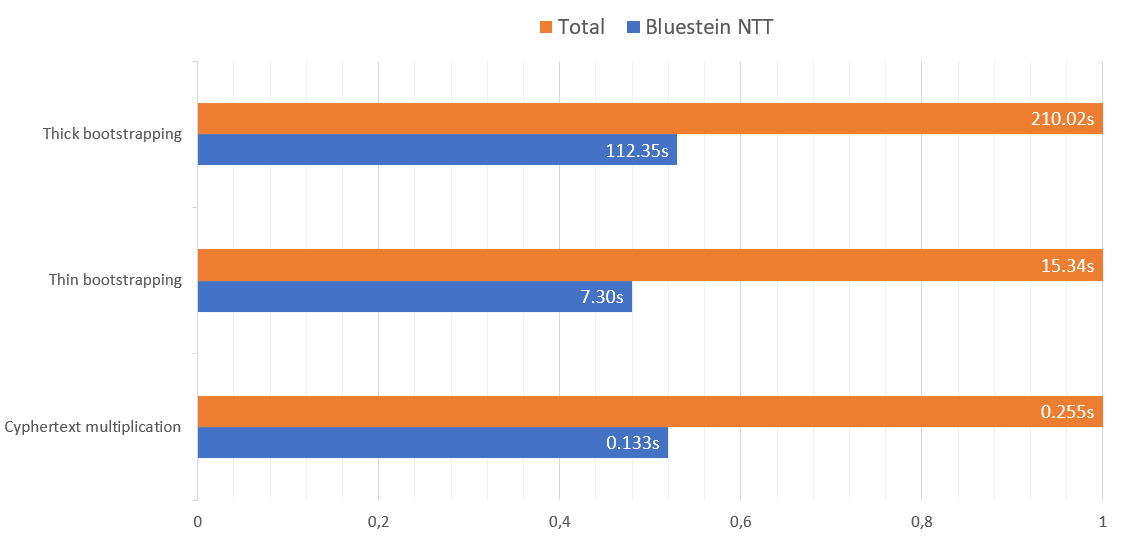
\includegraphics[width=0.8\textwidth]{img/HElib.png}
\caption{Timing of common FHE operations in HElib}
\label{fig:helib_timing}
\end{figure}

\FloatBarrier

\section{Hardware Acceleration}

Hardware acceleration is a technique used to improve the performance of specific computing tasks by offloading them from a general-purpose CPU to specialized hardware. Two common approaches to hardware acceleration are Field-Programmable Gate Arrays (FPGAs) and Application-Specific Integrated Circuits (ASICs).

\begin{itemize}
\item{\textbf{FPGAs}}
are reconfigurable semiconductor devices that allow creation of custom digital circuits. Unlike traditional ASICs, FPGAs can be programmed and reprogrammed to implement specific functions, making them highly adaptable for a wide range of tasks. While FPGAs provide flexibility, they may consume more power and have higher latencies compared to ASICs.

\item{\textbf{ASICs}}
are custom-designed integrated circuits optimized for a particular application or task. Unlike FPGAs, ASICs are fixed and cannot be reprogrammed after manufacturing. ASICs can achieve much higher performance than FPGAs and are ideal for high-volume production. However, ASIC development is much more expensive and has much longer design cycles compared to FPGA development.
\end{itemize}

In this thesis, we will use an FPGA to accelerate polynomial multiplication for polynomials with a degree that is not a power of two. Few hardware architectures have been explored to accelerate polynomial multiplication for this type of polynomials. Wu et al. \cite{9937536} explored an hardware architecture to accelerate the NTT using Bluestein's algorithm and Hsu and Shien \cite{9181192} proposed an hardware architecture based on the prime factor FFT algorithm and Rader's algorithm.


\chapter{Preliminaries and Algorithms}

In this chapter we first present the notations and basic definitions used in this thesis. Then, we delve into the BGV FHE scheme as used in the software library HElib and the basic concepts used in number theoretic transform (NTT). In the three following sections we focus on algorithms for NTTs of non power-of-two size, we introduce Bluestein's algorithm, Rader's algorithm and the prime-factor FFT algorithm (PFA), and show how they can be used to speed up the NTT computation. In the last section an algorithm based on a combination of PFA and Rader's algorithm is explored. An hardware implementation using this PFA-Rader algorithm is discussed in more detail in chapter \ref{chapter:hardware_implementation}.

\section{Definitions}
We use $\mathbb{Z}_q$ to denote the ring of integers with $q$ elements, also known as integers modulo $q$. In case $q$ is a prime number, $\mathbb{Z}_q$ forms a finite field. Elements in a ring are denoted by lowercase letters. Vectors of are expressed in bold $\mathbf{x} = \left \langle x_1, x_2, x_3, \ldots, x_{n-1}, x_n  \right \rangle$. The $i$-th component of vector $\mathbf{x}$ is specified as $x_i$.
\\\\
We use $\ast$ to represent the convolution operation between two vectors, whereas $\odot$ represents element wise multiplication. 
\\\\
$\omega$ is an $N$-th root of unity in $\mathbb{Z}_q$ if it satisfies the equation $\omega^N=1$. If additionally $\omega$ satisfies $\omega^m \neq 1$ for $m=1, 2, \ldots, m-1$ then it is said to be a primitive root of unity.
\\\\
$e \in \mathbb{Z}_q$ is an idempotent if it satisfies the equation $e^2 = e$. Two idempotents $e_1$ and $e_2$ are orthogonal if $e_1 e_2 = e_2 e_1 = 0$.


\section{The BGV Scheme}
The BGV encryption scheme is a fully homomorphic encryption (FHE) scheme that allows arbitrary computations on encrypted data without decrypting it. It was proposed by Zvika Brakerski, Craig Gentry, and Vinod Vaikuntanathan in 2011 \cite{BGV} and is based on the hardness of the Ring Learning with Errors (RLWE) problem \cite{app10175732}\cite{cryptoeprint:2012/230}. The BGV scheme supports addition and multiplication of ciphertexts, as well as scalar operations and rotations. The BGV scheme also allows for packing multiple plaintexts into a single ciphertext using the Chinese Remainder Theorem (CRT), which enables parallel processing and efficient homomorphic evaluation \cite{FHEsimd}.
\\\\
The BGV scheme operates on polynomials over cyclotomic rings. The plaintext space of the BGV scheme consists of vectors of integers modulo a plaintext modulus, which can be larger than 2. The ciphertext space of the BGV scheme consists of vectors of polynomials modulo a ciphertext modulus, which is a large integer that determines the security level and the noise budget. An important feature of the BGV scheme is the concept of modulus switching. A freshly encrypted ciphertext starts at encryption level $L$ and the encryption level gradually moves down as we perform homomorphic computations. With each encryption level $l$ a modulus $q_l$ is associated. Modulus switching helps to reduce the noise growth because when we switch the modulus from $q_l$ to $q_{l-1}$ with $q_{l-1} > q_l$ the noise term of the ciphertext is reduced by the ratio $\frac{q_l}{q_{l-1}}$. When we reach the smallest modulus $q_0$ at encryption level 0, the noise can no longer be reduced. At this point the ciphertexts needs to either be decrypted or Gentry's bootstrapping method\cite{10.1145/1536414.1536440} needs to be employed to enable further computation.
\\\\
In the implementation of the BGV scheme within HElib, a series of small machine-word sized prime numbers ${p_0, p_1, p_2, \ldots, p_L}$ are used to construct moduli as follows:\cite{cryptoeprint:2014/873} 
\[q_l = \prod_{i=0}^{i=l} p_i\]
The BGV scheme involves various operations with integer polynomials, such as modular multiplications, additions, and Frobenius maps. To increase efficiency, the polynomials used in these operations are represented using the DoubleCRT format. This format represents a polynomial as a collection of polynomials, each computed modulo a small primes $p_l$, with each individual polynomial further represented in evaluation form. In this evaluation form, a polynomial is described as a vector containing its values at primitive $N$-th roots of unity within the finite field $\mathbb{Z}_{p_l}$. Using this representation, polynomial multiplication simplifies to pointwise multiplication that can be performed in linear time. The transformation between coefficient representation, where the polynomial is expressed as a list of its coefficients, and evaluation representation involves using the Number Theoretic Transform (NTT). The NTT happens to be the most time-consuming step for calculations in HElib, therefore the hardware acceleration in this thesis will focus on optimizing this operation specifically.

\subsection{Parameters for Homomorphic SIMD}
As shown by Smart and Vercauteren\cite{FHEsimd} multiple smaller values can be packed into a single plaintext. This allows for efficient SIMD (Single Instruction Multiple Data) operations on encrypted data, as performing an operation on the entire ciphertext corresponds to performing that operation on each packed value individually. HElib makes extensive use of this technique to achieve better performance, however HElib imposes strong restrictions on the parameter $m$, which denotes the number of coefficients in the plaintext polynomial. This causes useful values of $m$ to have few divisors. Halevi and Shoup\cite{cryptoeprint:2014/873}  used a brute force search method to identify possible values for $m$, a selection of their results is shown in Table \ref{table:parameter_m}. Especially $m=21845$ and $m=65535$ will turn out to be very good choices for the algorithm described in section \ref{section:pfa_rader_alg}.

\begin{table}[h!]
\caption{Bootstrappable values for parameter $m$}
\label{table:parameter_m}
\centering
\begin{tabular}{|l|r|r|r|r|r|} 
\hline
cyclotomic ring m & 21845        & 35113        & 42799    & 49981   & 65535 \\ \hline \hline
m factorization   & $127\cdot17\cdot5$ & $73\cdot37\cdot13$ & $337\cdot127$ & $331\cdot151$ & $127\cdot17\cdot5\cdot3$ \\ \hline
number of slots   & 1024         & 864          & 2016     & 1650    & 2048 \\
 \hline
\end{tabular}
\end{table}

\FloatBarrier

\section{Number Theoretic Transform}

The number theoretic transform (NTT) generalizes the discrete Fourier transform (DFT) over $\mathbb{Z}_p$ where $p$ is prime.
It provides efficient algorithms for polynomial multiplication. \cite{cryptoeprint:2016/504}
$Z_p$ is a finite field, so there exists a primitive $N$-th root of unity if $N$ divides $p-1$.
Let $\omega$ be a primitive $N$-th root of unity then the N-point NTT $\mathbf{X}=\mathcal{N}\left(\mathbf{x}\right)$ is defined as:

\begin{equation}
\label{eq:ntt}
X_k = \sum_{n=0}^{N-1} x_n \omega^{nk} \qquad k=0,\ldots,N-1
\end{equation}

The inverse NTT $\mathbf{x}=\mathcal{N}^{-1}\left(\mathbf{X}\right)$ is defined as:

\begin{equation}
x_n = N^{-1}\sum_{k=0}^{N-1} X_k \omega^{-nk} \qquad k=0,\ldots,N-1
\end{equation}

Since $\omega$ is an N-th root of unity we have $\omega^{-nk} = \omega^{(N-k)n}$. This means an inverse NTT can be computed using a forward NTT by reversing the order of the elements in $\mathbf{X}$ as follows: $\left \langle X_0, X_1, X_2, \ldots, X_{N-2}, X_{N-1}  \right \rangle \rightarrow \left \langle X_0, X_{N-1}, X_{N-2}, \ldots, X_2, X_1 \right \rangle$.
\\\\
Because of the similarity between the NTT and DFT, any FFT algortihm can also be used for calculating the NTT.
The only modification that needs to be made is that $e^{-\frac{j2\pi}{N}}$ is replaced by $\omega$. \cite{1162555}
In the following sections the modifications to specific algorithms will be discussed in more detail.

\subsection{Polynomial Multiplication}
Polynomial multiplication is an important operation in lattice-based cryptography. Plaintext and ciphertext spaces are usually polynomial rings. To efficiently perform polynomial multiplication we use the negative wrapped convolution. \cite{cryptoeprint:2015/382} If we consider $\mathbf{a}$ and $\mathbf{b}$ two polynomials of degree N with coefficients in $\mathbb{Z}_q$, $\omega, \psi \in \mathbb{Z}_q$ with $\omega$ a primitive N-th root of unity and $\psi^2 = \omega$. We can calculate the polynomial product $\mathbf{c} = \mathbf{a} \cdot \mathbf{b}$ as follows:

\begin{equation} 
\begin{split}
\mathbf{a}^\prime &= \left \langle a_0, \psi a_1, \psi^2 a_2, \ldots, \psi^{N-1} a_{N-1} \right \rangle \\
\mathbf{b}^\prime &= \left \langle b_0, \psi b_1, \psi^2 b_2, \ldots, \psi^{N-1} b_{N-1} \right \rangle \\
\mathbf{c}^\prime &= \mathcal{N}^{-1}\left\{\mathcal{N}\left\{ \textbf{a}^\prime \right\} \odot \mathcal{N}\left\{ \textbf{b}^\prime \right\} \right\} \\
\mathbf{c} &= \left \langle c_0^\prime, \psi^{-1} c_1^\prime, \psi^{-2} c_2^\prime, \ldots, \psi^{-\left(N-1\right)} c_{N-1}^\prime \right \rangle \\
\end{split}
\end{equation}

By using the NTT for polynomial multiplication all other operations involved become simple pointwise multiplication. Polynomial multiplication can be computed in quasilinear time when an FFT algorithm is used for the NTTs.

\section{Bluestein's algorithm}

Bluestein's algorithm permits to efficiently compute the DFT of any size, including prime sizes. \cite{1162132}
We show below how this algorithm can be used to compute the NTT.
\\\\
Begin with the definition of the NTT (\ref{eq:ntt})
\[X_k = \sum_{n=0}^{N-1} x_n \omega^{nk} \qquad k=0,\ldots,N-1\]
If we replace $nk$ in the exponent by

\begin{equation}
nk = \frac{k^2}{2}+\frac{n^2}{2}-\frac{\left(k-n\right)^2}{2}
\end{equation}

we obtain:

\begin{equation}
X_k = \omega^{\frac{k^2}{2}}\sum_{n=0}^{N-1} \left(x_n \omega^{\frac{n^2}{2}}\right) \omega^{-\frac{(k-n)^2}{2}} \qquad k=0,\ldots,N-1
\end{equation}

This summation can be expressed as the convolution of two sequences $a_n$ and $b_n$ as follows:

\begin{equation}
\begin{split}
& a_n = x_n \omega^{\frac{n^2}{2}} \\
& b_n = x_n \omega^{-\frac{n^2}{2}} \\
& X_k = b_k^{-1} \left(\sum_{n=0}^{N-1} a_n b_{k-n} \right) \qquad k=0,\ldots,N-1
\end{split}
\end{equation}

The convolution is computed by a pair of NTTs using the convolution theorem (\ref{eq:conv_theorem_bluestein}).

\begin{equation}
\label{eq:conv_theorem_bluestein}
\mathbf{a} \ast \mathbf{b} = \mathcal{N}^{-1}\left\{\mathbf{A}\odot \mathbf{B}\right\}
\end{equation}

The advantage here is that these NTTs do not have to be of length N. The convolution can be computed after zero-padding it to a length of at least $2N-1$.
By padding it to a power of two, the NTT can be computed efficiently using the Cooley-Tukey algorithm in $O\left(M\log_2 M\right)$, where $M$ is the padded length.
If the NTT of sequence $b_n$ is precomputed, the total number of multiplications needed for this convolution can be estimated as $M + 2 M\log_2 M$.

\section{Rader's algorithm}

Rader's algorithm permits to efficiently compute the DFT of prime sizes. \cite{1448407}
We show below how this algorithm can be used to compute the NTT.
\\\\
Begin with the definition of the NTT (\ref{eq:ntt})

\[X_k = \sum_{n=0}^{N-1} x_n \omega^{nk} \qquad k=0,\ldots,N-1\]

If $N$ is a prime number, then the set of integers modulo $N$, denoted as $\mathbb{Z}_N$, forms a finite field with $N$ elements. In this finite field, there exists a primitive root $g \in \mathbb{Z}_N$ such that for any non-zero element $n \in \mathbb{Z}_N$, there exists a unique exponent $q \in \{0, 1, 2, \ldots, N-2\}$ satisfying the equation: $n = g^q \pmod{N}$. Since every non-zero element in $\mathbb{Z}_N$ corresponds to a unique $q$ this forms a bijection from $q$ to non-zero $n$. In the same way $k = g^{-p} \pmod{N}$, with k a non-zero element in $\mathbb{Z}_N$ and $p \in \{0, 1, 2, \ldots, N-2\}$ forms a bijection from $p$ to non-zero $k$. If we rewrite the NTT using these indices we get:

\begin{equation}
\begin{split}
& X_0 = \sum_{q=0}^{N-1} x_n
& X_{g^{-p}} = x_0 + \sum_{q=0}^{N-2} x_{g^q} \omega^{g^{-\left(p-q\right)}} \qquad p=0,\ldots,N-2
\end{split}
\end{equation}

This summation can be expressed as the convolution of two sequences $a_q$ and $b_q$ as follows:
\begin{equation}
\begin{split}
& a_q = x_{g^q} \\
& b_q = \omega^{g^{-q}} \\
& X_{g^{-p}} = x_0 + \left(\sum_{n=0}^{N-2} a_q b_{p-q} \right) \qquad p=0,\ldots,N-2
\end{split}
\end{equation}

Just like in Bluestein's algorithm this convolution can be performed by a pair of NTTs by using the convolution theorem (\ref{eq:conv_theorem_rader}).

\begin{equation}
\label{eq:conv_theorem_rader}
\mathbf{g} \ast \mathbf{h} = \mathcal{N}^{-1}\left\{\mathbf{G}\odot \mathbf{H}\right\}
\end{equation}
The difference here is that this convolution is of length $N-1$ instead of length $N$. It can again be zero padded to a length of at least $2(N-1)-1$, but if $N-1$ is already highly composite there are efficient FFT algorithms where padding isn't necessary. If $N-1$ is a power of two and the NTT of sequence $b_q$ is precomputed, the total number of multiplications needed for this convolution can be estimated as $\left(N-1\right) + 2 \left(N-1\right)\log_2 \left(N-1\right)$.

\subsection{An Optimization to Rader's Algorithm}
Rader's algorithm requires $N-1$ additions to compute $X_0 = \sum_{i=0}^{N-1} x_i$ and $N-1$ additions to add $x_0$ to each element of the convolution result. This number can be reduced to just two additions. We observe that

\begin{equation}
A_0 = \sum_{q=0}^{N-2} x_{g^q} = \sum_{i=1}^{N-1} x_i
\end{equation}

so $X_0$ can be computed as $X_0 = x_0 + A_0$. If $\mathbf{C} = \mathbf{A} \odot \mathbf{B}$, then adding $x_0$ to $C_0$ before the inverse NTT corresponds to adding $x_0$ to each element of $\mathbf{c}$. Algorithm \ref{alg:rader} describes our implementation of Rader's algorithm with these modifications. Note that we excluded the final reversed re-indexing step.

\begin{algorithm}
\caption{Optimized Rader's Algorithm}\label{alg:rader}
\KwData{$\mathbf{x}$, sequence of $N$ integers}
\KwResult{$\mathbf{X} = \mathcal{N}\left(\mathbf{x}\right)$}
$\mathbf{x^\prime} \gets$ RaderPermutation$([x_1, x_2,\ldots, x_{N-1}])$\;
$\mathbf{A} \gets \mathcal{N}(\mathbf{x^\prime})$\;
$X_0 \gets A_0 + x_0$\;
$\mathbf{C} \gets \mathbf{B} \odot \mathbf{A}$\;
$C_0 \gets C_0 + x_0$\;
$[X_1, X_2,\ldots, X_{N-1}] \gets \mathcal{N}^{-1}\left(\mathbf{C}\right)$\;
\end{algorithm}

\section{Prime-Factor FFT Algorithm (PFA)}

The Prime-Factor FFT algorithm (PFA) transforms a discrete Fourier transformation (DFT) with a size of $N = N_1 N_2$ into a two-dimensional DFT with dimensions $N_1 \times N_2$. \cite{1671829} It is important that $N_1$ and $N_2$ are integers that have no common factors. By applying PFA recursively, the smaller DFTs of size $N_1$ and $N_2$ can be computed. For instance, if $N$ had three coprime factors $N = N_1 N_2 N_3$ a three-dimensional $N_1 \times N_2 \times N_3$ FFT is obtained. The factorization is similar to Cooley-Tukey but has the advantage that no multiplications with twiddle factors are required. However, PFA has the disadvantage that it only works if $N$ has coprime factors, so it is useless for powers of two, and a more complex re-indexing based on the Chinese remainder theorem (CRT) is used. When the smaller transforms can not be factored anymore another FFT algorithm has to be used.

To explain this re-indexing in more detail we start with the definition of the NTT (\ref{eq:ntt})
\[X_k = \sum_{n=0}^{N-1} x_n \omega^{nk} \qquad k=0,\ldots,N-1\]

PFA relies on a factorization of $N = N_1 N_2$ with $N_1$ and $N_2$ coprime.
According to the Chinese remainder theorem we can find central orthogonal idempotents $e_1$ and $e_2$ such that $e_1^2 = e_1 \pmod{N}$,  $e_2^2 = e_2 \pmod{N}$, $e_1 e_2 = 0 \pmod{N}$ and $e_1 + e_2 = 1 \pmod{N}$.

Choosing $\omega_1 = \omega^{e_1}$ and $\omega_2 = \omega^{e_2}$ we have $\omega_1 \omega_2 = \omega^{e_1} \omega^{e_2} = \omega$. Note that $\omega^n$ is cyclic in $N$ while $\omega_1^n$ and $\omega_2^n$ are cyclic in $N_1$ and $N_2$ respectively. The NTT can be rewritten as:

\begin{equation}
\begin{split}
X_k &= \sum_{n=0}^{N-1} x_n \omega^{nk} = \sum_{n=0}^{N-1} x_n \left( \omega_1 \omega_2 \right)^{nk} = \sum_{n=0}^{N-1} x_n \omega_1^{(n \mod N_1)(k \mod N_1)} \omega_2^{(n \mod N_2)(k \mod N_2)} \\
&= \sum_{n_1=0}^{N_1-1}\sum_{n_2=0}^{N_2-1} x_{e_1 n_1 + e_2 n_2} \omega_1^{n_1 (k \mod N_1)} \omega_2^{n_2(k \mod N_2)}
\end{split}
\end{equation}

After re-indexing $x_{n_1,n_2} = x_{e_1 n_1 + e_2 n_2}$ and $X_{k_1,k_2} = X_{k_1 e_1 + k_2 e_2}$ we obtain the two dimensional DFT (\ref{eq:2D_DFT})

\begin{equation}
\label{eq:2D_DFT}
X_{k_1,k_2} = \sum_{n_1=0}^{N_1-1}\sum_{n_2=0}^{N_2-1} x_{n_1,n_2} \omega_1^{n_1 k_1} \omega_2^{n_2 k_2}
\end{equation}

Figure \ref{fig:pfa_illustration} illustrates how an NTT of size $15$ can be re-expressed as a two-dimensional NTT of size $5 \times 3$. In this case we have $N = 15, N_1 = 5, N_2 = 3, e_1 = 10$ and $e_2 = 6$. When computing the NTT of the matrix, the same values are be obtained as when computing the NTT of the sequence directly. The result will be scrambled unless a reverse re-indexing is be performed. To calculate convolutions the scrambled result can be used, for other applications it will need to be unscrambled first.

\begin{figure}[h]
\setcounter{MaxMatrixCols}{20}
\resizebox{\textwidth}{!}{
$\begin{bmatrix}
x_0 & x_1 & x_2 & x_3 & x_4 & x_5 & x_6 & x_7 & x_8 & x_9 & x_{10} & x_{11} & x_{12} & x_{13} 
\end{bmatrix} \rightarrow \begin{bmatrix}
x_0 & x_{10} & x_{5} \\ 
x_6 & x_1 & x_{11} \\ 
x_{12} & x_7 & x_2 \\ 
x_3 & x_{13} & x_8 \\ 
x_9 & x_4 & x_{14}
\end{bmatrix}$
}
\caption{Illustration of re-indexing when $N = 15$.}
\label{fig:pfa_illustration}
\end{figure}


\section{Combined PFA-Rader Algorithm}
\label{section:pfa_rader_alg}

For an arbitrary N-point sequence, three different scenarios can be defined:
\begin{itemize}
  \item When N can be factored into coprime numbers $N_1$ and $N_2$, the problem of computing an N-point NTT can be reformulated using PFA into computing $N_2$ instances of an $N_1$-point NTT and $N_1$ instances of an $N_2$-point NTT.
  \item When N is not a prime number but a prime power, represented as $p^k$, the Cooley-Tukey FFT algorithm can be used. \cite{Cooley1965AnAF}
  \item When N is a prime number, the problem of computing the N-point NTT can be transformed using Rader's algorithm into computing two (N-1)-point NTTs.
\end{itemize}

Any of these algorithms will reduce the sizes of the NTTs to be performed. By recursively selecting the appropriate algorithm for each new size encountered, an efficient approach to performing NTTs of any size can be found. \cite{Parker1995UnusuallengthNT}
\\\\
Figure \ref{comparison_algorithm_multiplicatons} shows how this method compares to both direct application of Bluestein's algorithm and application of PFA followed by Bluestein for different bootstrappable parameters of the BGV-FHE scheme from Table \ref{table:parameter_m}. For this comparison it is assumed that each power-of-two length NTT requires $N \log N$ multiplications. Recursive application of PFA and Rader requires significantly less multiplications than Bluestein either directly or after PFA. 

\begin{figure}[h]
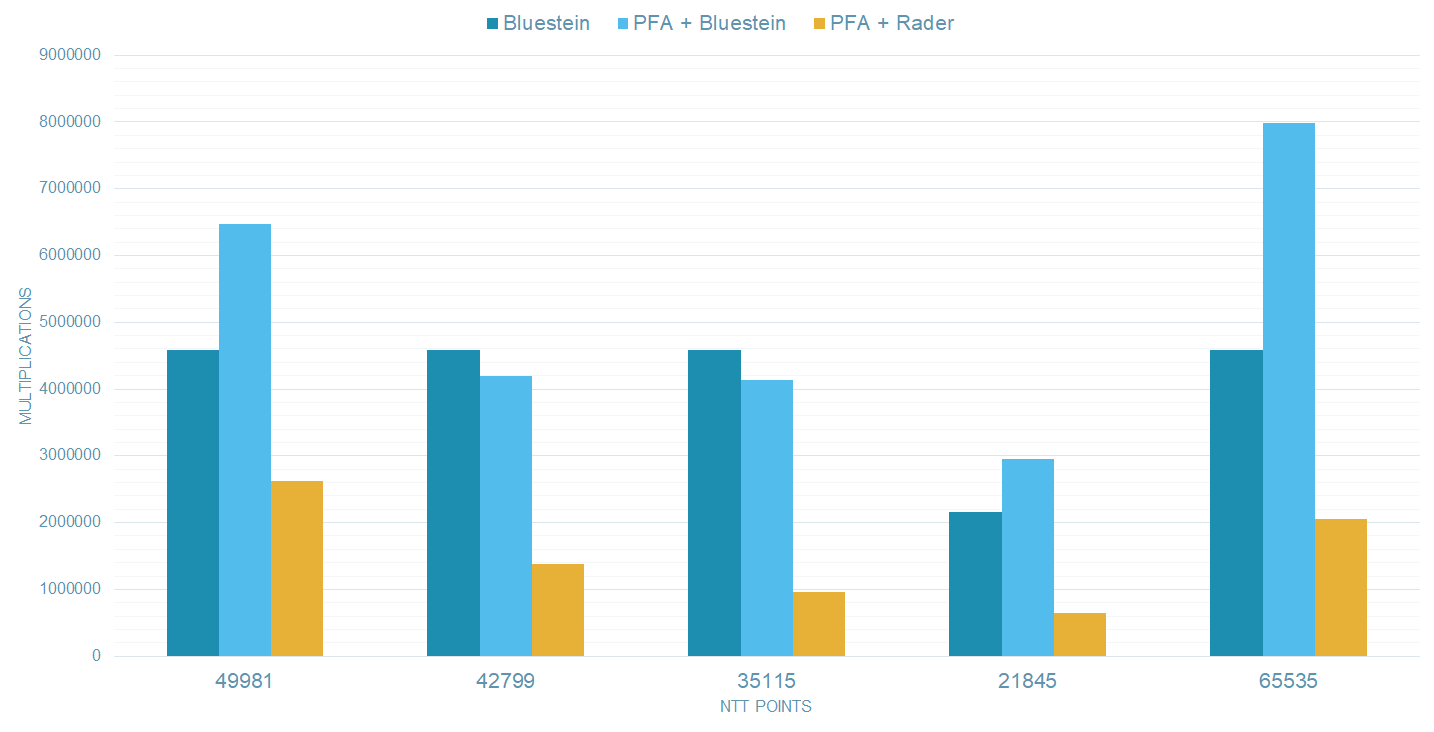
\includegraphics[width=\textwidth]{img/comparison_algorithm_multiplications.png}
\caption{Number of multiplications required to perform different NTT algorithms.}
\label{comparison_algorithm_multiplicatons}
\end{figure}

In the context of precomputing twiddle factors and precomputing the NTT of the sequence $b_n$ in Bluestein's algorithm or $b_q$ in Rader's algorithm, another important factor to consider is the size of the required lookup table. If Bluestein's algorithm is applied directly, the length of the NTT is at least doubled, this means $N$ twiddle factors need to be stored and $2N$ values of $B_n$. A single application of PFA reduces the number of twiddle factors from $N$ to $N_1 + N_2$, and number of $B_n$ values to $2\left(N_1 + N_2\right)$.
\\\\
Another thing to consider are the restrictions on the moduli that can be used in computing the NTT. A primitive N-th root of unity exist in the ring $\mathbb{Z}_p$ when $p$ is of the form $p = kN + 1$. Since different NTT length are used in the algorithm, a prime $p$ is required that satisfies this property for each length. Table \ref{table:moduli} shows the possible moduli for different bootstrappable parameters for both the PFA-Rader algorithm and Bluestein's algorithm. The table also includes the minimum number of bits needed to represent the first twenty possible values for $p$. Bluestein's algorithm generally requires longer word sizes.

\begin{table}[h!]
\caption{Possible moduli for PFA-Rader FFT and Bluestein FFT}
\label{table:moduli}
\centering
\begin{tabular}{|r|r|r|r|r|} 
 \hline
  & \multicolumn{2}{c|}{PFA-Rader} & \multicolumn{2}{c|}{Bluestein} \\
 \hline
 \multicolumn{1}{|c|}{N} & \multicolumn{1}{c|}{$p$} & \multicolumn{1}{c|}{n-bits} & \multicolumn{1}{c|}{$p$} & \multicolumn{1}{c|}{n-bits}  \\
 \hline
 49\,981 & $49\,481\,190k+1$ & 33 & $6\,551\,109\,632k+1$ & 41 \\ 
 42\,799 & $43\,141\,392k+1$ & 32 & $5\,609\,750\,528k+1$ & 41  \\
 35\,115 & $82\,169\,100k+1$ & 34 & $4\,602\,593\,280k+1$ & 39 \\
 21\,845 & $5\,592\,320k+1$ & 30 & $1\,431\,633\,920k+1$ & 38  \\
 65\,535 & $16\,776\,960k+1$ & 31 & $8\,589\,803\,520k+1$ & 40  \\ 
 \hline
\end{tabular}
\end{table}

Because of these advantages the hardware architecture will be based on the PFA-Rader algorithm rather than Bluestein. However, it is important not to forget that PFA-Rader also has drawbacks such as the high complexity and scrambled results.

\section{Conclusion}
In this chapter, we introduced the essential notations and definitions used throughout this thesis. We discussed the BGV Fully Homomorphic Encryption (FHE) scheme and its operations on polynomials over cyclotomic rings. The Number Theoretic Transform (NTT) was introduced as a fundamental operation for polynomial multiplication in lattice-based cryptography.
\\\\
We explored three key algorithms for NTT computation: Bluestein's algorithm, Rader's algorithm, and the Prime-Factor FFT algorithm (PFA). We highlighted how Bluestein's algorithm is versatile for handling various sizes of NTTs, Rader's algorithm efficiently handles prime-sized NTTs, and PFA decomposes NTTs into smaller ones. Additionally, we discussed the combination of PFA and Rader's algorithm, which provides an optimized approach for computing NTTs of different sizes, making it suitable for hardware implementation.
\\\\
By analyzing the number of multiplications and moduli constraints, we determined that the combined PFA-Rader algorithm offers advantages over Bluestein's algorithm. With these considerations in mind, the chosen hardware architecture, discussed in the next chapter, will be based on the PFA-Rader algorithm.

\chapter{Hardware Implementation}
\label{chapter:hardware_implementation}

Current state of the art software implementations of FHE still have very poor performance. When using the HElib software library, a single ciphertext multiplication takes multiple seconds and the bootstrapping operation that enables FHE can take multiple minutes. \cite{cryptoeprint:2018/244} This is too slow to be practical for many applications. NTT computations account for approximately half of the time spent in the multiply and bootstrapping operations.  Therefore the hardware accelerating done in this thesis serves as a good starting point.
\\\\
 We designed an architecture to target the specific parameter choice of the 21845-th cyclotomic polynomial, which is a practical parameter for BGV. As shown in the previous chapter, section \ref{section:pfa_rader_alg}, the parameter 21845 has ideal properties for use with the Prime-Factor FFT algorithm (PFA) and Rader’s algorithm. This chapter will start with a general overview of the datapath and control logic designed in this thesis. In the next sections we will discuss the challenges with implementing a complex algorithm in hardware. At the end of the chapter we will discuss the results and compare our implementation to other NTT accelerators.

\section{Hardware Platform}
The device targeted for this thesis is the Alveo U250 Data Center Accelerator Card. 

\section{Overview}

We implement the PFA-Rader algorithm as detailed in section \ref{section:pfa_rader_alg} for a 21845-point NTT. PFA transform the task of computing one 21845-point NTT into multiple small NTTs of sizes 257, 17 and 5. All of these small NTTs are subsequently transformed using Rader's algorithm into convolutions with a precomputed constant $\mathbf{B}$ of length 256, 16 and 4 respectively and some extra additions, see algorithm \ref{alg:rader}. Each convolution requires a forward power-of-two-size NTT and an inverse NTT. The inverse NTT is preforming using the same hardware as the forward NTT, only the twiddle factors are different. The multiplication with a scaling factor $N^{-1}$ is avoided by absorbing it into $\mathbf{B}$. To maximize effective use of resources the same hardware that computes the 256-point NTTs is also used for the smaller sized NTTs and for the pointwise multiplication with $\mathbf{B}$. A similar architecture is possible for a 65535-point NTT, for any other parameter this approach would not work.
\\\\
\subsection{Datapath Overview}
The hardware architecture is based on vector processors. Vector processors excel at exploiting data parallelism by performing operations on large one-dimensional arrays of data called vectors. The data is streamed through a highly pipelined vector processor, ideally without any stall cycles. Given that the processor is pipelined, a high clock rate can be applied. And since there are no wait states, all processing elements are optimally used. This result is a very efficient implementation.
\\\\
The proposed hardware architecture, as depicted in Figure \ref{fig:hardware_overview}, utilizes vectors composed of 257 32-bit words, resulting in a total size of 8224 bits. This size corresponds to the largest dimension in the resulting $257 \times 85$ matrix obtained through PFA.
\\\\
Each vector in this architecture can represent either one row of the matrix or three columns. As the vectors pass through the datapath, either one recursive stage of the Cooley-Tukey FFT algorithm or 128 pointwise multiplications can be computed. Each functional unit in the architecture is designed to handle a throughput of one vector per cycle. The NTT unit consists of 128 radix-2 butterfly units. These units can be configured to perform either a butterfly operation or only a multiplication and modular reduction.
\\\\
To achieve the required memory bandwidth, the system employs 257 individually addressable memory banks. The rows of the matrix are stored in a staggered manner, ensuring that each element of a row or column resides in a different memory bank. An address generator determines the read and write addresses, while barrel shifters eliminate and reapply the offset caused by row staggering.

\begin{figure}[h]
\centering
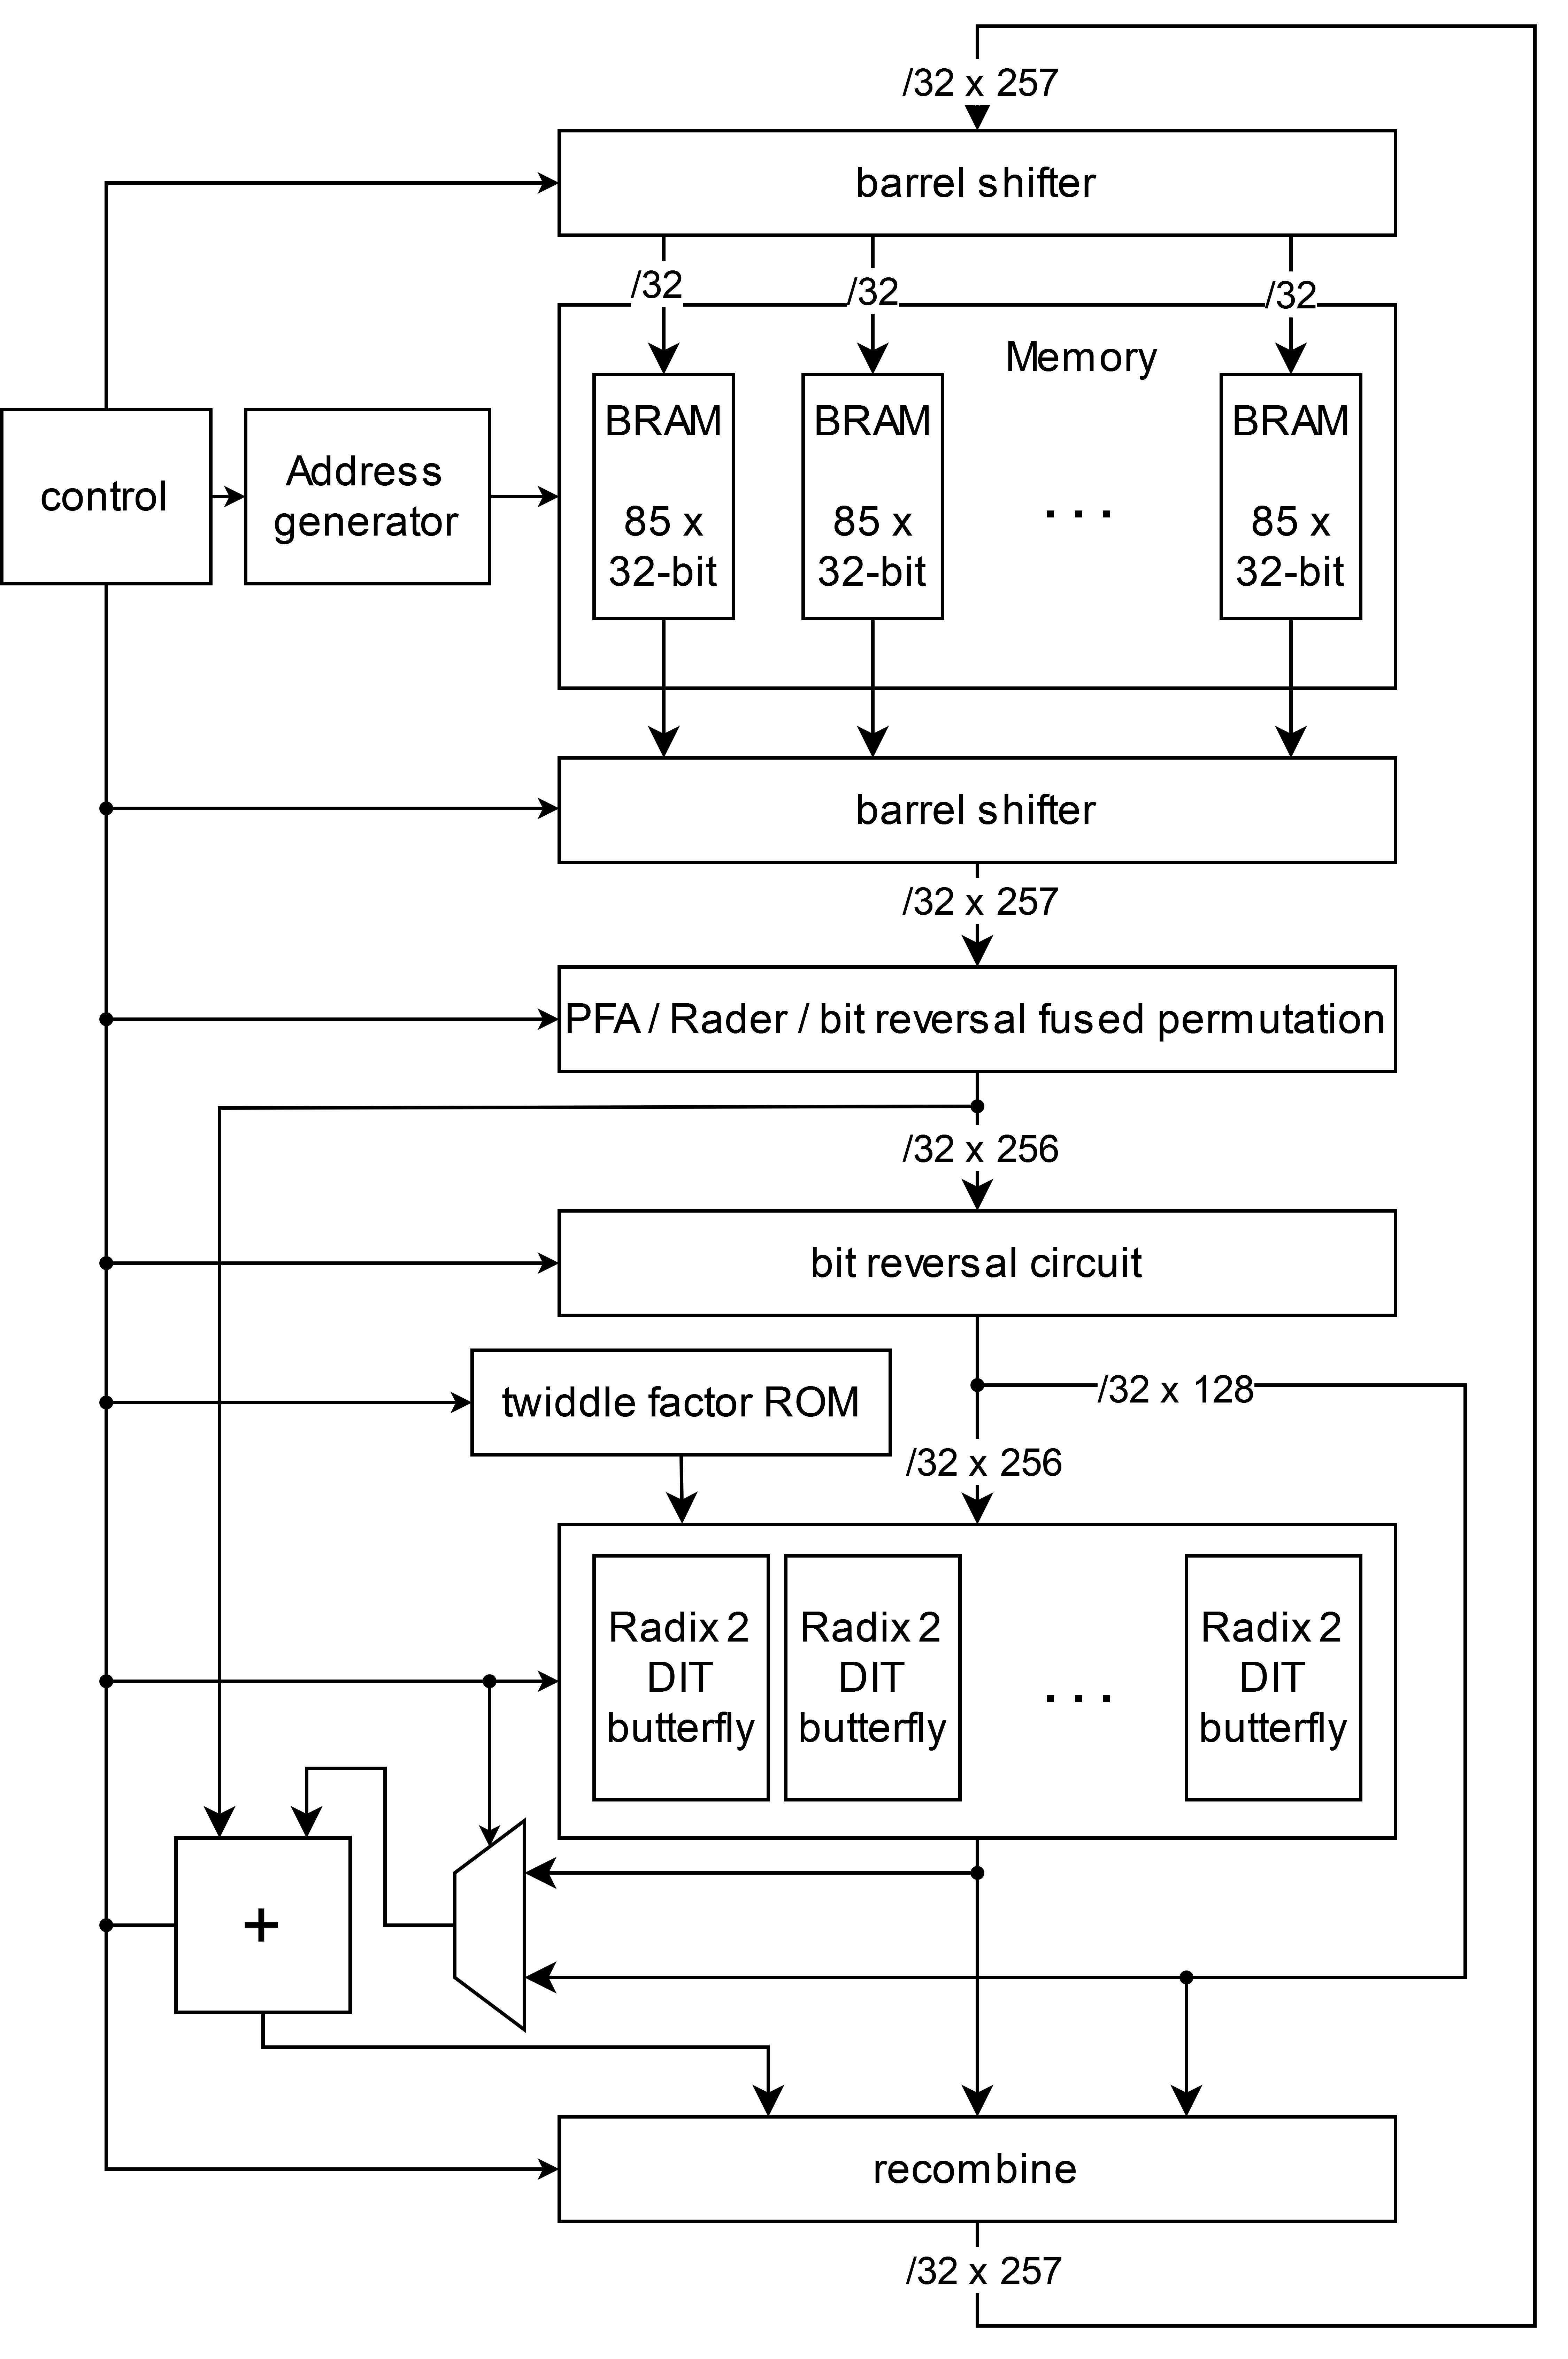
\includegraphics[width=0.9\textwidth]{img/architecture.png}
\caption{Proposed FFT hardware architecture}
\label{fig:hardware_overview}
\end{figure}

\FloatBarrier

\subsection{Control Flow}
\label{section:control_flow}
Figure \ref{fig:state_diagram} shows the controller state diagram, which governs the processing of a three-dimensional grid of size $257 \times 17 \times 5$ obtained through PFA. The outer loop in the controller contains seven distinct states, including the initial idle state. Additionally, there are three state variables: \emph{axis}, \emph{row} and \emph{step}. \emph{axis} refers to the direction in which we are iterating through the grid, \emph{row} refers to the index of the current row that is being processed, and \emph{step} to the current stage in the Cooley-Tukey algorithm. The output of the controller depends on both the current state and the current axis.
\\\\
Each stage of the NTT computation is performed on all rows along one dimension of the matrix before moving on to the next stage. Iterating over the NTT stages in the inner loop and over the rows in the outer loop would result in undesirable pipeline stalls, because there is a data dependency between two stages of the NTT computation. The iteration order is different for the Multiply part 1 and Multiply part 2 states where an operation on the same row can be performed in two subsequent cycles, since there is no data dependency between these two operations. Because some of the data required for part 2 would be overwritten an additional temporary storage would be needed. However, this extra storage is not required if both operations are performed in subsequent cycles. Which is why we iterate over the rows in the outer loop here.
\\\\
The only instance where the pipeline stalls is in the final state, where it waits for all NTTs along the current axis to complete. This stall is necessary when transitioning from rows to columns because there is a data dependency between each row and column. While stalling during the switch between axes of the $5 \times 17$ NTTs is not strictly necessary, the delay is negligible in the total computation, so it is left as is.

\begin{figure}[h]
\centering
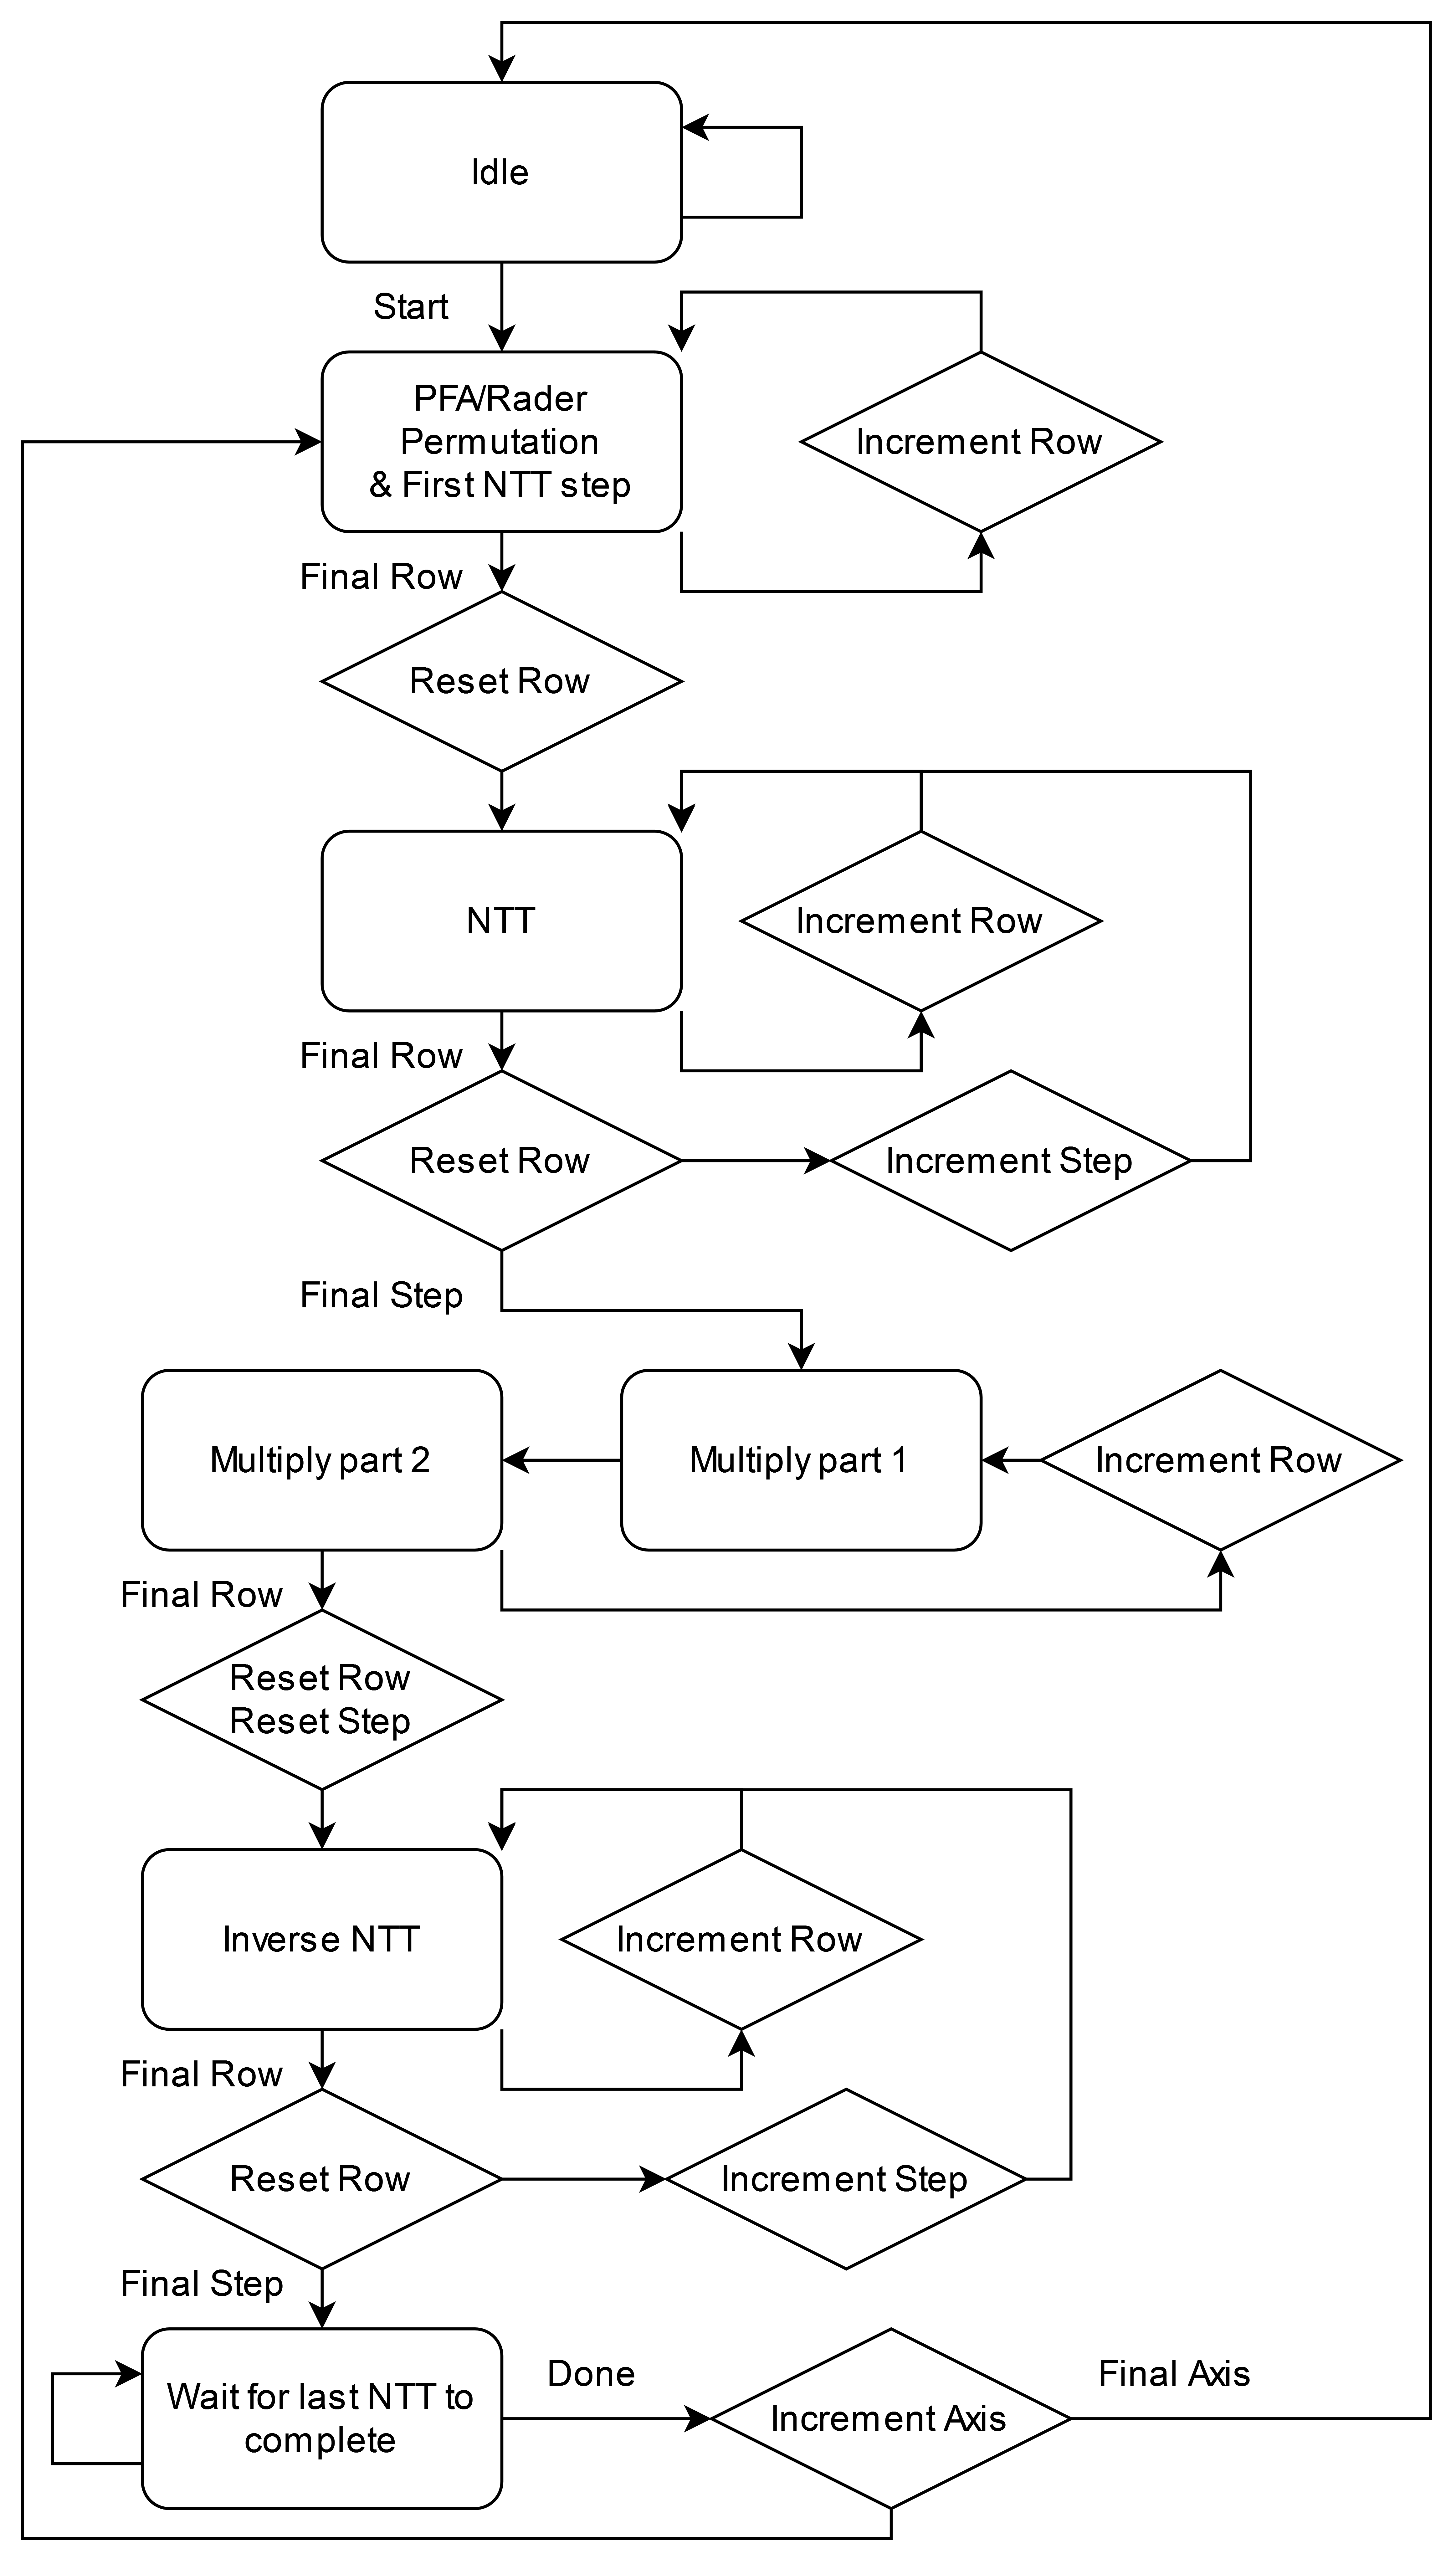
\includegraphics[width=0.85\textwidth]{img/control_flow.png}
\caption{Control state diagram.}
\label{fig:state_diagram}
\end{figure}

\FloatBarrier

\section{PFA and Rader Permutations}
\subsection{Efficient Memory Design}
PFA is used to re-express the NTT of size $N = 21845$ as a two-dimensional NTT over a $257\times 85$ matrix. The matrix elements are stored in 257 Block RAMs (BRAMs) on the FPGA. Each BRAM consists of 85 32-bit words and has separate read and write ports, meaning that a vector of 257 32-bit words can be read from or written to the memory every cycle.
\\\\
However, there is a challenge when accessing the matrix elements in parallel. If each column of the matrix is stored in a separate BRAM, it allows accessing an entire row in parallel. But it prevents accessing multiple elements from a column simultaneously. On the other hand, if each row of the matrix is is stored in a separate BRAM, it allows accessing multiple elements from a column in parallel but restricts accessing an entire row simultaneously.
\\\\
To overcome this limitation and enable parallel access to both rows and columns, a staggered memory arrangement is used. In this arrangement, the matrix rows are stored in a staggered manner, where each row is offset by one BRAM from the previous row. This means that each element of a column, as well as each element of a row, is stored in a different BRAM. The illustration in Figure \ref{fig:staggered_memory} demonstrates this arrangement using a smaller example, showing a 7×5 matrix. Each color in the figure represents a unique column of the matrix. Important to note is the separation of elements in different BRAMs for both rows and columns.

\begin{figure}[h]
\centering
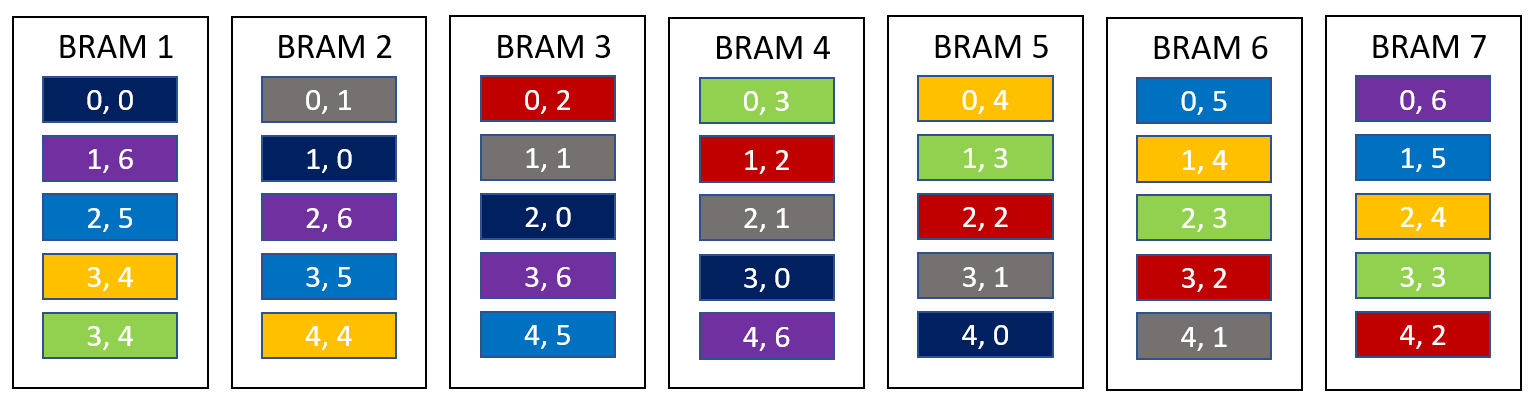
\includegraphics[width=0.8\textwidth]{img/staggered_memory.png}
\caption{Illustration of staggered rows in memory, each color represents a column in the PFA matrix.}
\label{fig:staggered_memory}
\end{figure}

\FloatBarrier

To facilitate reading from and writing to memory with the required offsets, two circular shift circuits are needed: one at the write ports and another at the read ports of the memory. These circular shift circuits allow circularly shifting 32-bit words across lanes in a vector of length 257, meaning each word can be shifted to a different position within the vector. To achieve a throughput of one vector per cycle a barrel shifter is used. The design of a barrel shifter for a vector of length 5 is shown as an example in Figure \ref{fig:barrel_shifter}, a similar design is used for the vector of length 257. The barrel shifter is implemented using 1-bit 2-to-1 multiplexers.

\begin{figure}[h]
\centering
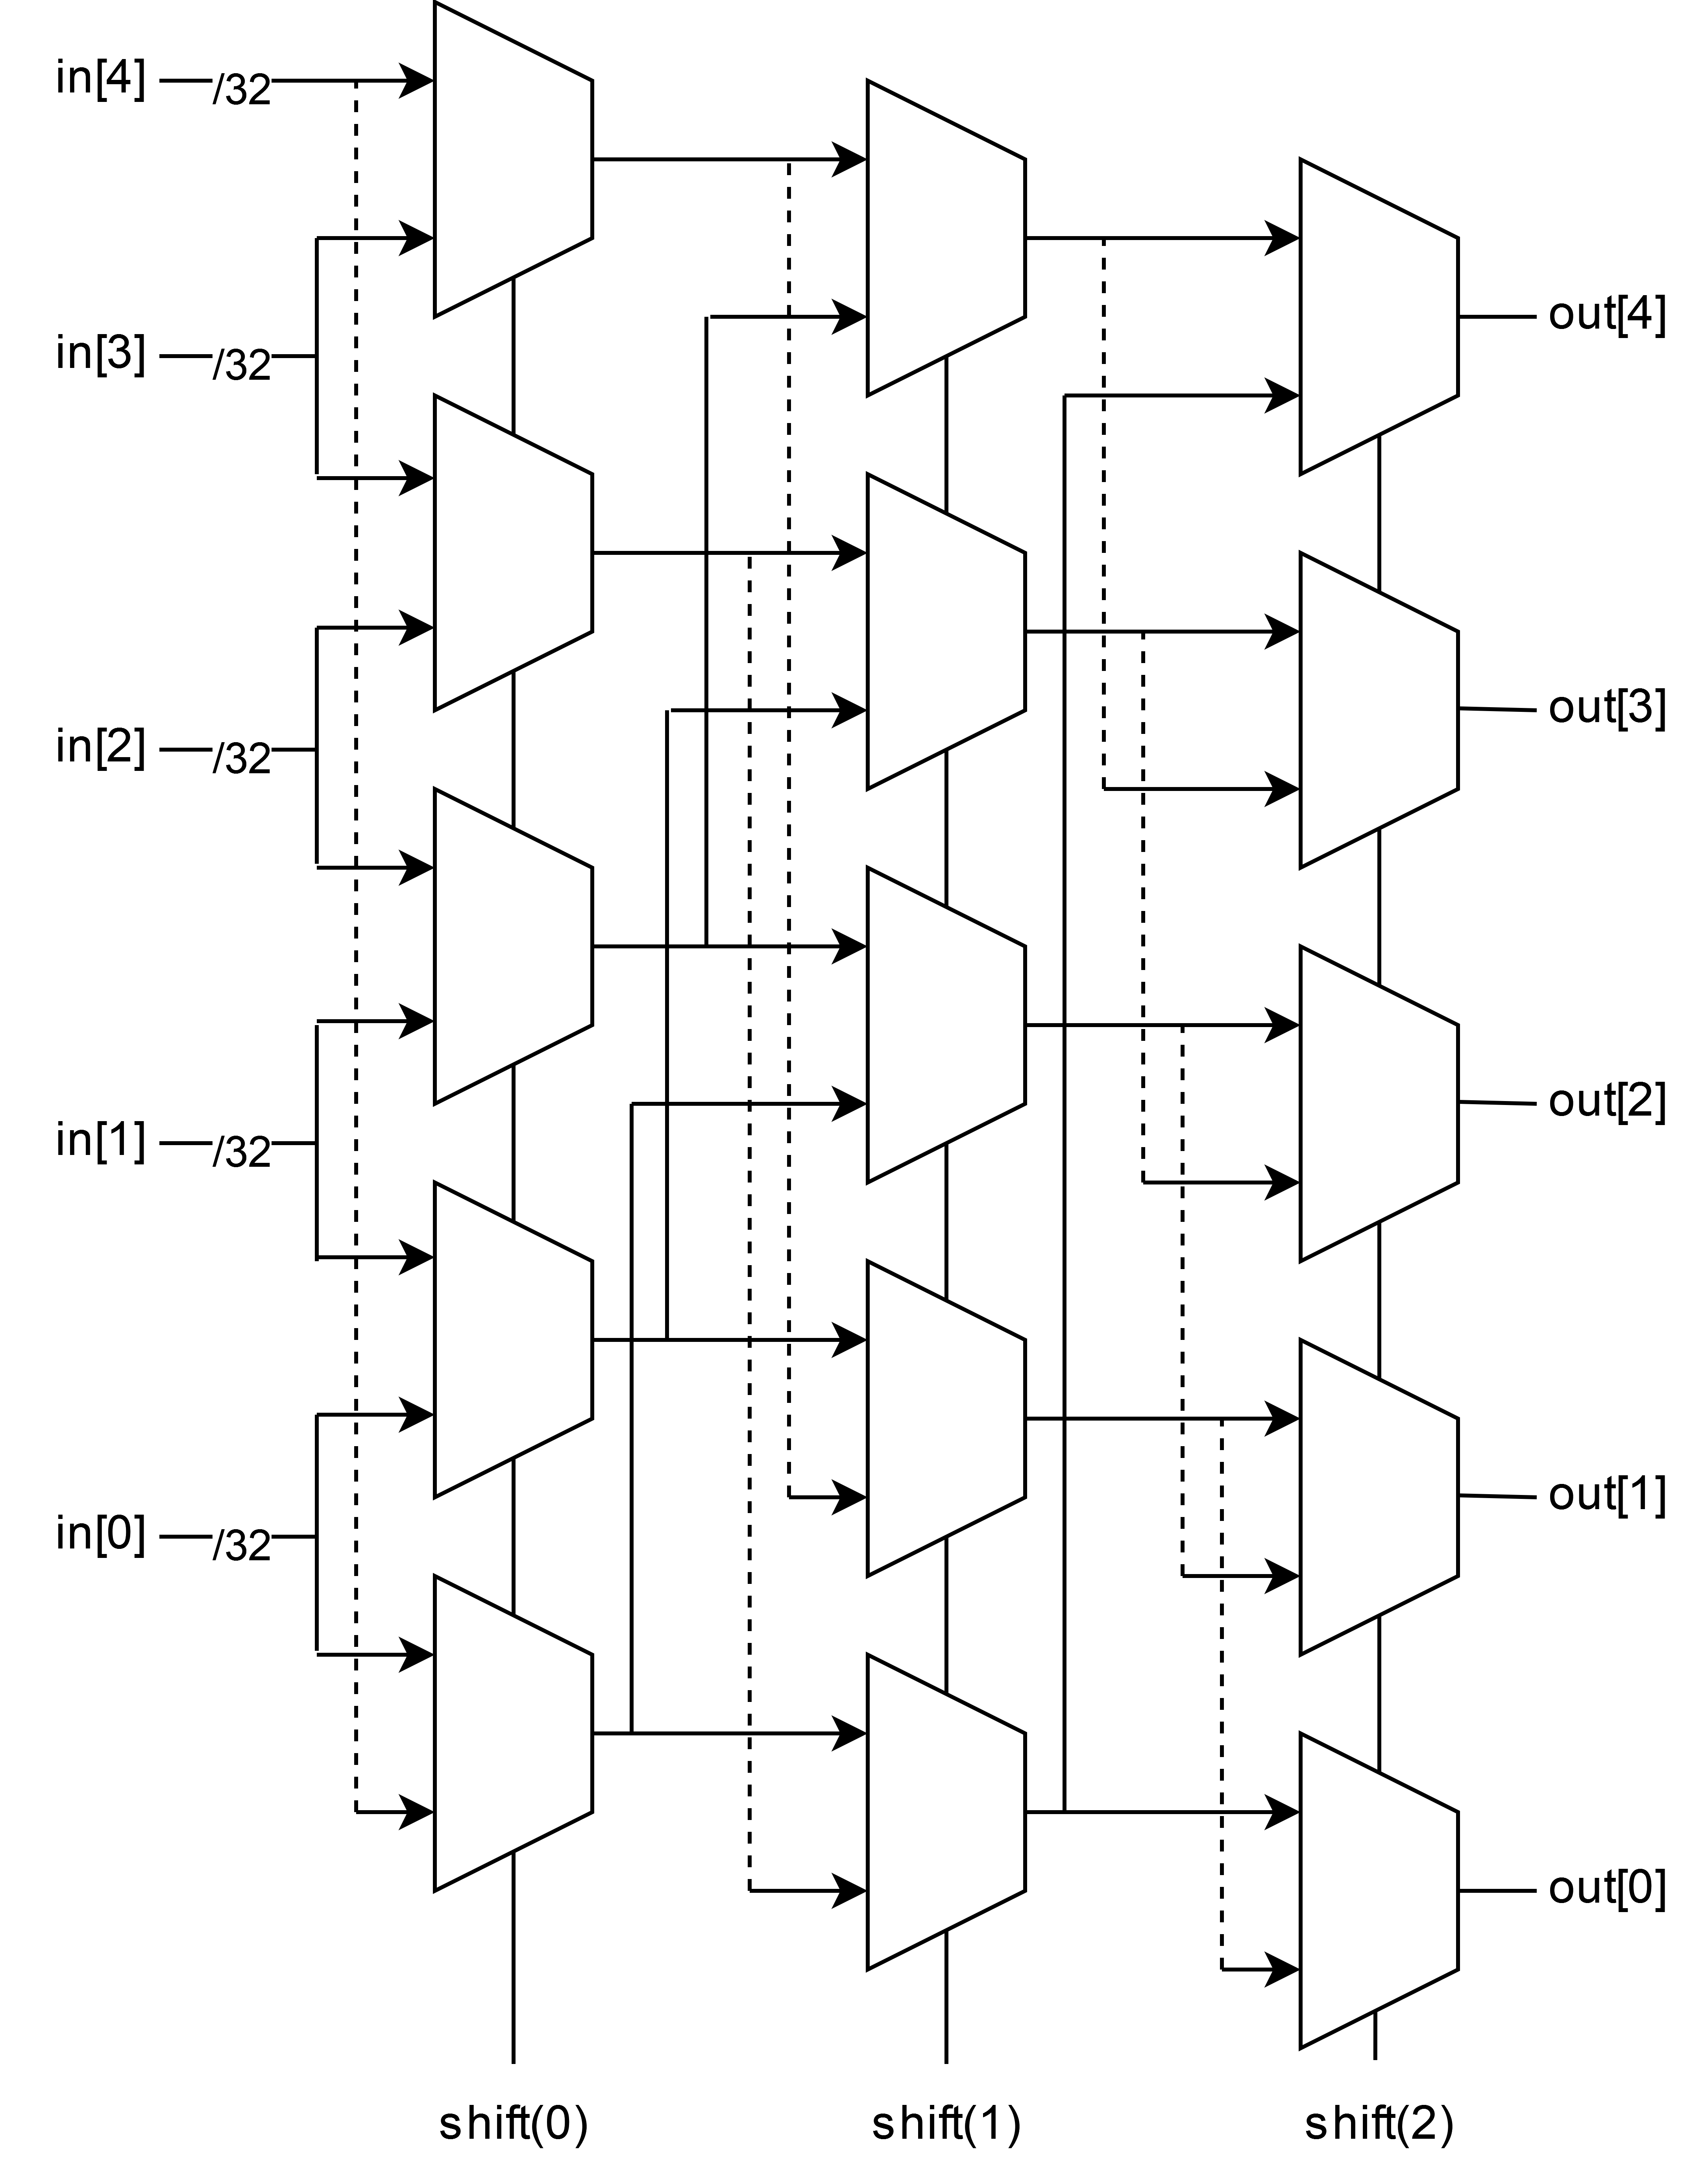
\includegraphics[width=0.7\textwidth]{img/barrel_shifter.png}
\caption{Barrel shifter design.}
\label{fig:barrel_shifter}
\end{figure}

\FloatBarrier

The number of multiplexers required can be calculated using the formula:
\[w \cdot N \cdot \left \lceil \log_2 N \right \rceil\]
where:
\begin{itemize}
\item{$w$ represents the number of bits in each word (32 bits)}
\item{$N$ represents the length of the vector (257 in this case)}
\end{itemize}
Since one 6-input Look-Up Table (LUT6) on the FPGA can implement two 2-to-1 multiplexers, the total number of LUTs required to implement both barrel shifters is determined to be 74016 LUTs.
\\\\
Finally, figure \ref{fig:mem_design} shows the combined memory with barrel shifters design.

\begin{figure}[h]
\centering
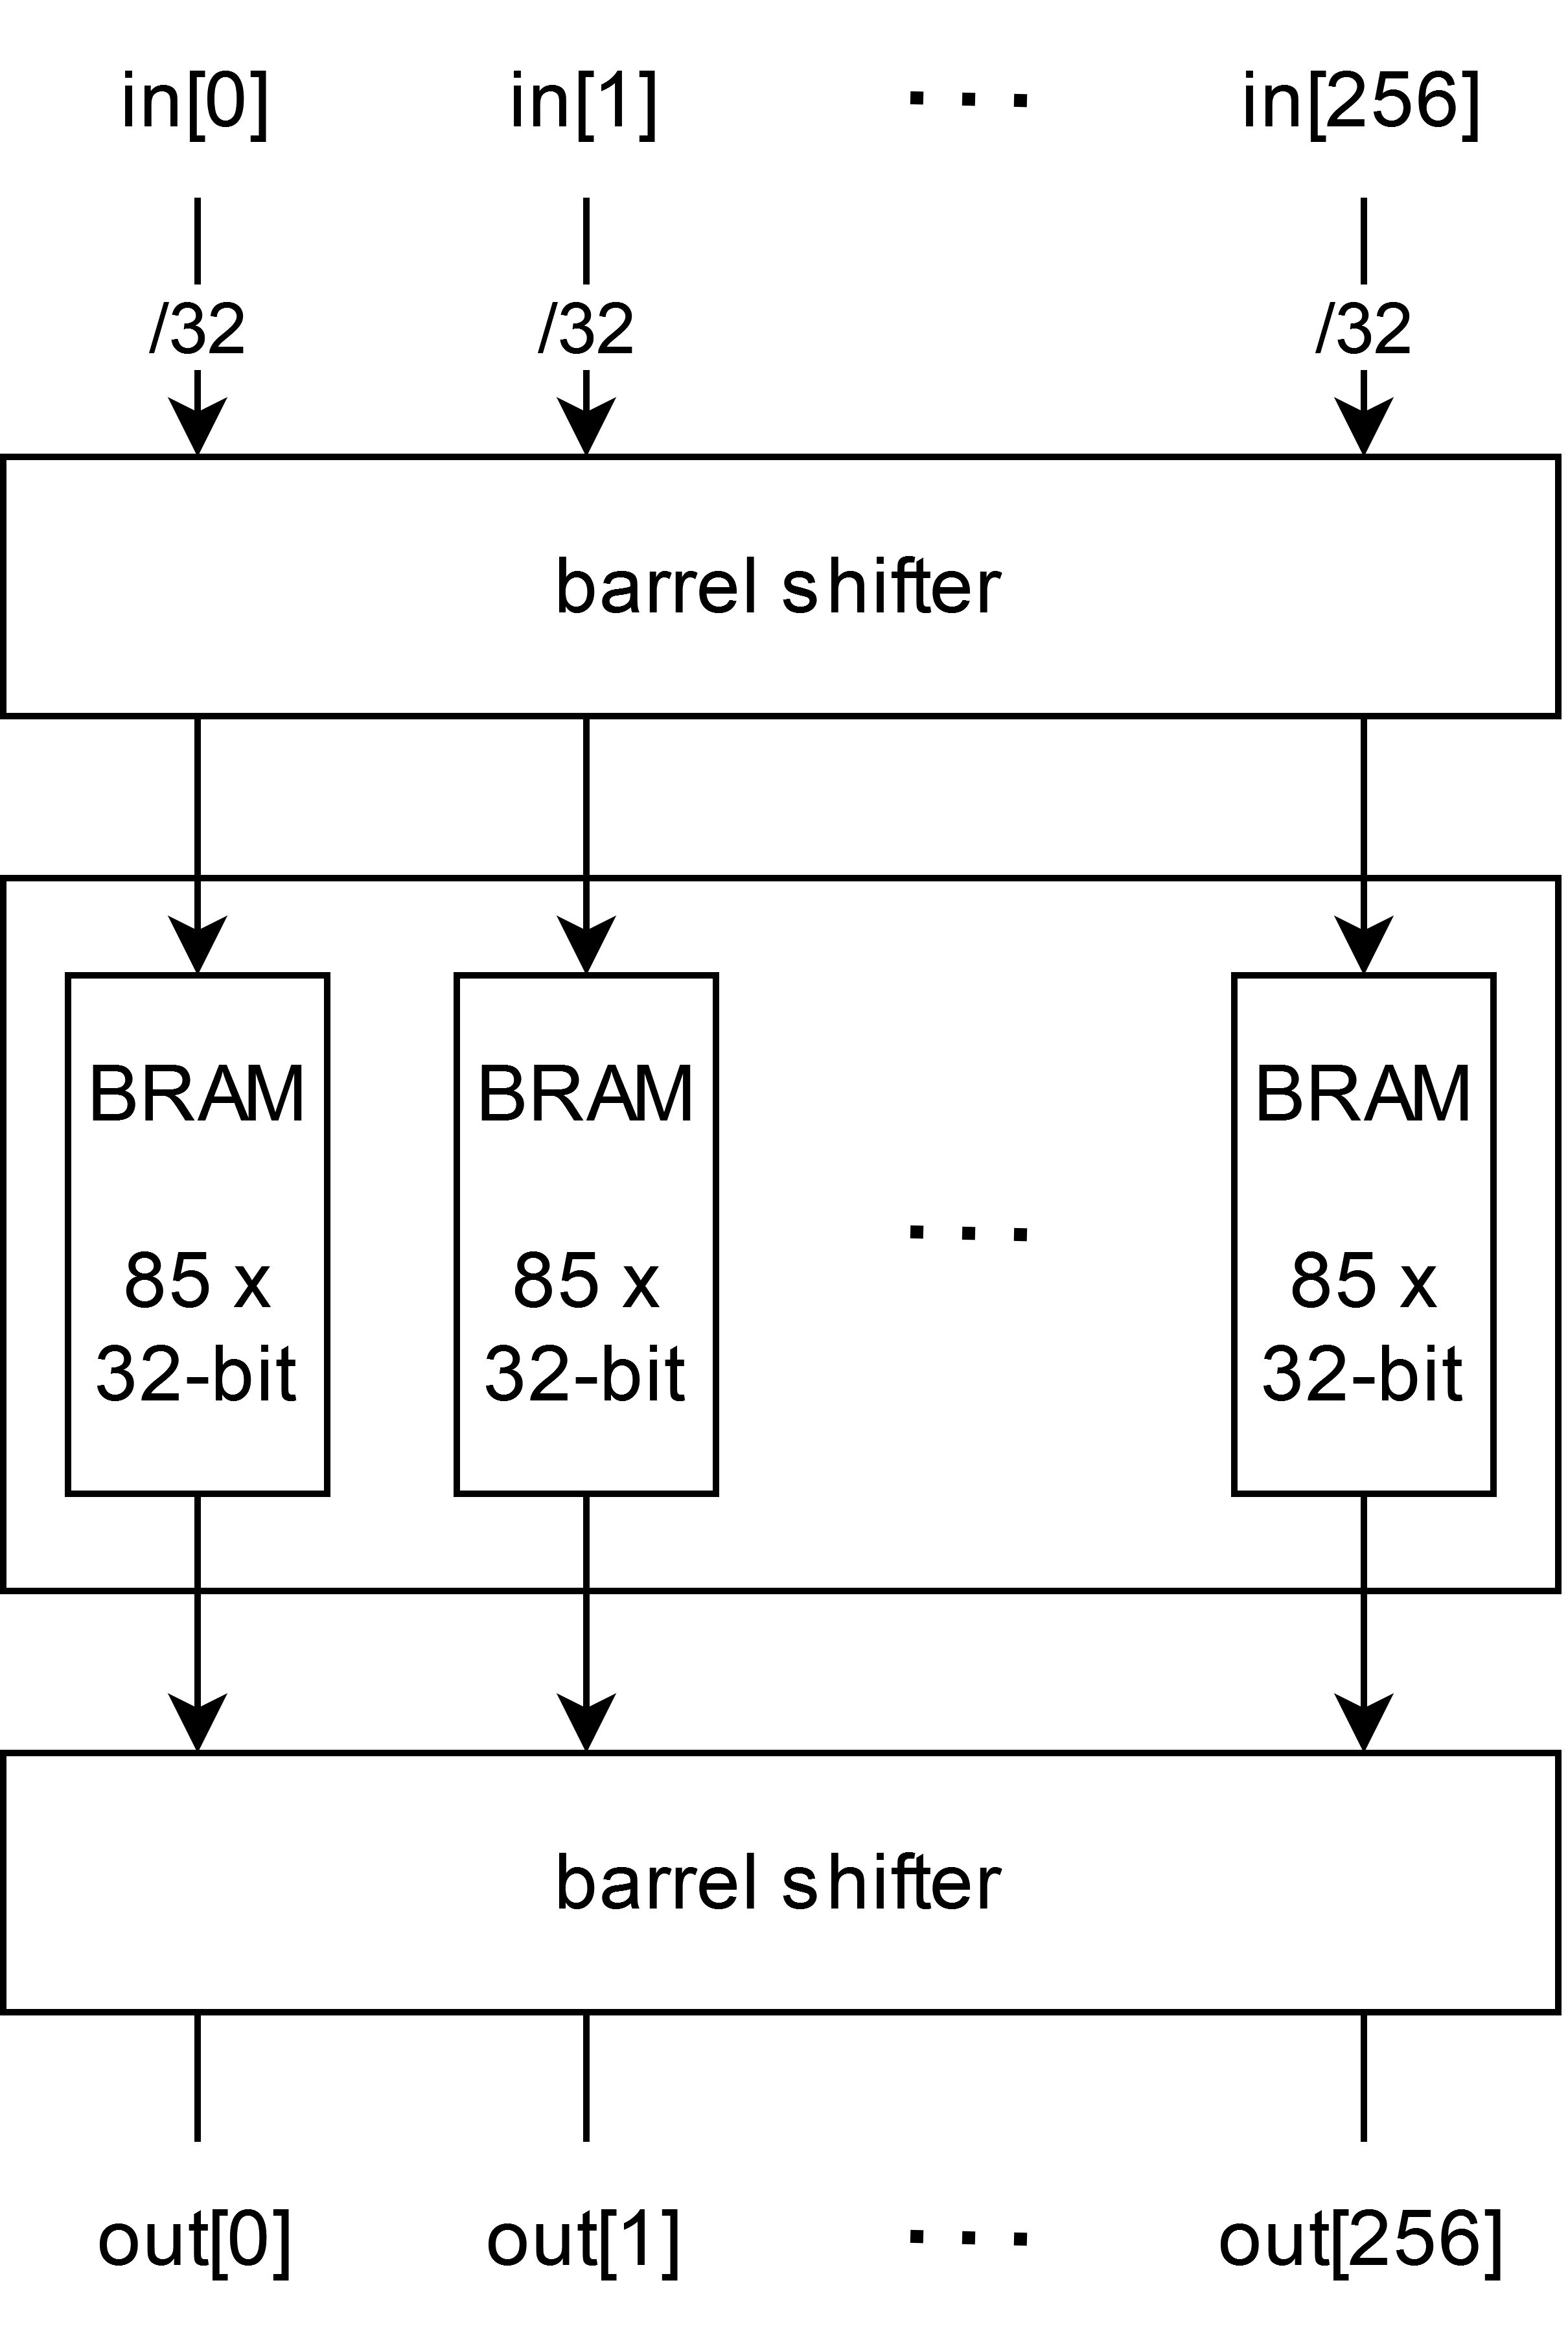
\includegraphics[width=0.5\textwidth]{img/mem_design.png}
\caption{Implementation of memory using BRAMs and circular shift circuits.}
\label{fig:mem_design}
\end{figure}

\FloatBarrier

\subsection{Combining permutations}
The NTTs of size 85 over the columns are re-expressed as a two-dimensional NTT over a $17\times 5$ matrix. A permutation is used that creates a vector with every row of the matrix arranged behind one another. However, there is another permutation needed to obtain a vector that concatenates the columns instead of the rows. This permutation corresponds to transposing the matrix. By applying this additional permutation, the resulting vector will have the elements from each column arranged in sequence.
\\\\
The NTTs of size 257, 17 and 5 are computed using Rader's algorithm. In Rader's algorithm, the first element of each row (with sizes 257, 17, and 5) in the vector needs to be removed. A permutation removes the first points from the NTT vectors and fills the gaps with subsequent elements. The removed first points are collected and placed at the end of the vector. An additional permutation is required for re-indexing in Rader's algorithm. This permutation is different for each NTT size (257, 17, and 5).
\\\\
Furthermore, a bit-reversal permutation is necessary because the radix-2 DIT (Decimation in Time) butterflies expect the initial input in a bit-reversed order.
\\\\
It seems that there are many permutations involved, but by combining certain permutations, their total number can be reduced to six. These six permutations are as follows:

\begin{samepage}
\begin{enumerate}
\item{Collecting first points, Rader's re-indexing, and bit-reversed ordering for size row 257}
\item{PFA permutation combined with removing first points, Rader's re-indexing, and bit-reversed ordering for row size 17}
\item{Matrix transpose combined with removing first points, Rader's re-indexing, and bit-reversed ordering for row size 5}
\item{Removing first points for row size 257}
\item{Removing first points for row size 17}
\item{Removing first points for row size 5}
\end{enumerate}
\end{samepage}

To select one permutation from the reduced set of six, a 6-to-1 multiplexer is used. Two 5-input Look-Up Tables (LUT5) on the FPGA can implement a 1 bit 6-to-1 multiplexer. For a vector of 257 32-bit words, the number of LUTs would be 16448 LUTs. However, due to the fact that some elements are assigned the same index in different permutations, the actual number of LUTs needed for the implementation could be lower than this initial estimate.

\section{Vectorized Cooley-Tukey FFT}
The Cooley-Tukey FFT algorithm, specifically the radix-2 decimation-in-time (DIT) variant, works by breaking down a Discrete Fourier Transform (DFT) of a larger size $2n$ into two smaller transforms of size $n$. These smaller transforms are then combined using mathematical operations called "butterflies," which involve computing smaller DFTs of size 2 that are multiplied with roots of unity known as "twiddle factors". Figure \ref{fig:dit_fft} shows a butterfly diagram for an 8-point FFT algorithm, which illustrates how the inputs and outputs are connected for each stage during the computation. It is evident that the same hardware used for computing an FFT of size $2n$ can also be used for computing two FFTs of size $n$ by just omitting the final stage of the FFT and adjusting the twiddle factors. This property allows for reusing the hardware resources efficiently. Therefore, the focus of the design is on implementing a 256-point FFT, and the same hardware is used for computing 16-point and 4-point FFTs.

\begin{figure}[h]
\centering
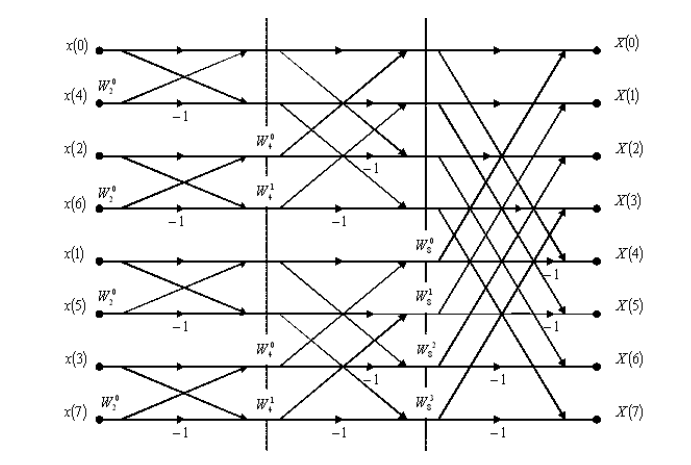
\includegraphics[width=0.8\textwidth]{img/dit_fft.png}
\caption{Butterfly diagram for radix-2 DIT FFT algorithm from Pace et al. \cite{ditfftimg}}
\label{fig:dit_fft}
\end{figure}

\FloatBarrier

\subsection{Bit-reversal permutations}
In the Cooley-Tukey FFT algorithm, after each stage of butterfly operations, the data needs to be reordered to prepare for the next stage. This particular reordering is known as "bit-reversal". Bit-reversal permutation ensures that the data is in the correct order for each recursive stage of the FFT algorithm.
The bit-reversal permutation essentially reverses the binary representation of the indices of the data points. Consider a simple example with a 4-point FFT:
\\\\
Original indices: 0, 1, 2, 3
\\\\
Binary representations: 00, 01, 10, 11
\\\\
Bit-reversed indices: 0, 2, 1, 3
\\\\
The bit-reversed indices are obtained by reversing the order of bits in the binary representation of the original indices. As seen in the example, the indices are reordered from (0, 1, 2, 3) to (0, 2, 1, 3) after the bit-reversal step.
\\\\
Since the bit-reversal permutations need to be performed between each recursive stage of the FTT algorithm, they also require a throughput of one vector per cycle. To achieve this throughput a specialized bit-reversal circuit is used. The circuit is implemented as a series of eight bit-reversal permutations of increasing length $\{2, 4, 8, 16, 32, 64, 128, 256\}$. Multiplexers are used to select either the permuted vector or the non-permuted vector. This bit-reversal circuit can perform length 1, 2, 4, 8, 16, 32, 64, 128 and 256 permutations which are all required by the radix-2 Cooley-Tukey algorithm. Since each bit-reversal permutation is an involution, a permutation can be removed by reapplying the same permutation. The bit-reversal circuit is implemented using 1-bit 2-to-1 multiplexers.
\\\\
The number of multiplexers required can be calculated using the formula:
\begin{equation}
w \cdot \left( N \cdot \log_2(N) - \frac{5N}{2} + 2 \right)
\end{equation}
where:
\begin{itemize}
\item{$w$ represents the number of bits in each word (32 bits)}
\item{$N$ represents the length of the vector (256 in this case)}
\end{itemize}
Since one 6-input Look-Up Table (LUT6) on the FPGA can implement two 2-to-1 multiplexers, the total number of LUTs required to implement the bit-reversal circuit is determined to be 22560 LUTs.

\section{Butterfly units}
\label{section:butterfly_units}

The implementation utilizes a total of 128 butterfly units, enabling the execution of a single stage of the 256-point FFT per cycle. With the 128 butterfly units, it is also possible to calculating one stage of sixteen FFTs of size 16, or one stage of sixty-four FFTs if size 4. The design of one such butterfly unit is shown in Figure \ref{fig:dit_rader_butterfly}. 

\begin{figure}[h]
\centering
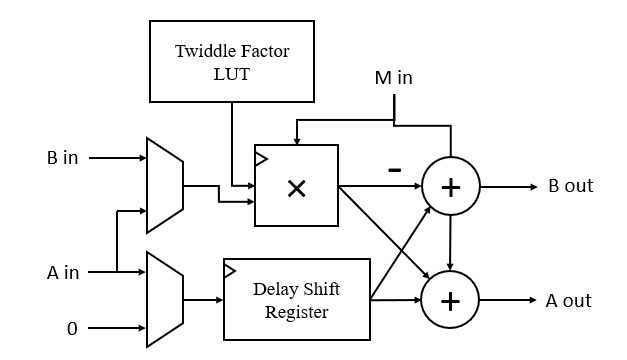
\includegraphics[width=0.8\textwidth]{img/dit_rader_butterfly.png}
\caption{Implementation of radix-2 DIT FFT butterfly}
\label{fig:dit_rader_butterfly}
\end{figure}

\FloatBarrier

One of the inputs is always a constant twiddle factor, therefore each butterfly unit has a lookup table containing the twiddle factors $\omega$ for the radix-2 FFT. The butterfly unit makes use of a word-level Montgomery modular multiplier implementation from Mert et al. \cite{9171507}. The multiplier takes $A$, $B$ and $m$ as input and calculates the output $A \cdot B \cdot R^{-1} \pmod m$, where $R = 2^K$ is the Montgomery reduction residual and $K$ is the number of bits in the modulus (in our case 32). This means an extra multiplication with $R$ is required to obtain $A \cdot B \pmod m$. However, this extra multiplication can be omitted by precomputing the twiddle factors in the lookup table as $\omega \cdot R \pmod m$. The multiplier is fully pipelined and has a throughput of one multiplication and modular reduction per cycle with a latency of eleven cycles. The algorithm is originally designed for $N$-point NTTs where $N$ is a power of two and relies on the property that $2N$ is a power of two and that for any usable modulus $m = 1 \pmod{2N}$. In our case $N$ is not a power of two, but any usable modulus is of the form $m = 257 \cdot 17 \cdot 5 \cdot 256 \cdot k + 1$ with $k$ a positive integer. Therefore any usable modulus $m = 1 \pmod{256}$. In general the largest power of two that divides any of the NTT lengths can be used instead of $2N$. A shift register is used to match the latency of the modular multiplier for the other input. Figure \ref{fig:mod_add_sub} shows the design used for the final modular addition and subtraction.

\begin{figure}[h]
\centering
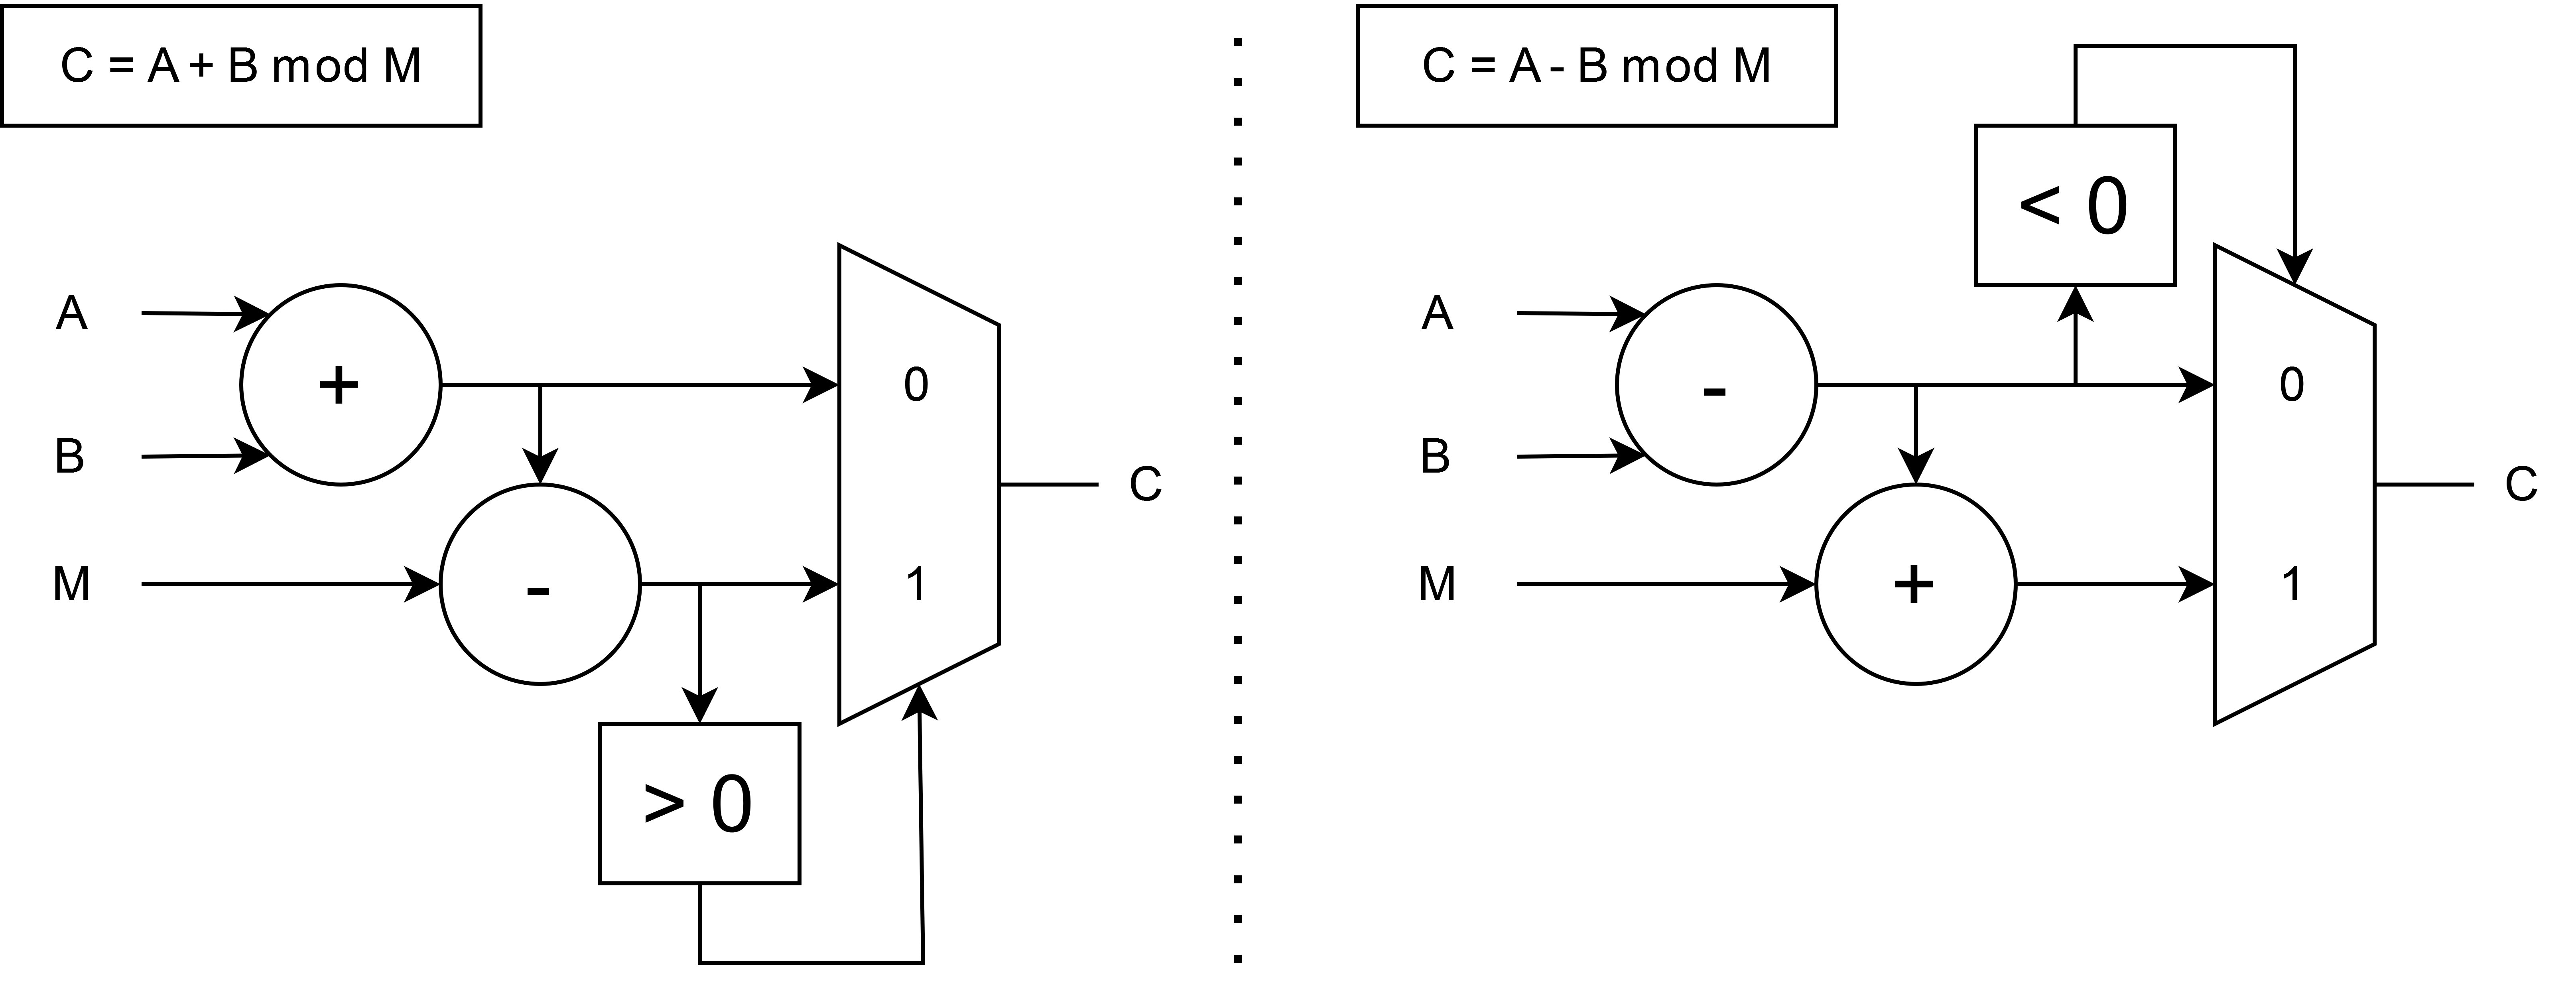
\includegraphics[width=1\textwidth]{img/mod_add_sub.png}
\caption{Design of modular adder and subtractor.}
\label{fig:mod_add_sub}
\end{figure}

\FloatBarrier

The convolution in Rader's algorithm requires a pointwise product to be computed. It would be inefficient to add more modular multipliers just for this operation, since they would be unused most of the time. Therefore, we reuse the multipliers in the butterfly units. One of the factors in the pointwise product is a precomputed constant, these constant factors can be stored in the lookup table that already contains the FFT twiddle factors. To multiply without the final addition a multiplexer is added at input A that allows to set one of the inputs of the addition to zero. Another multiplexer is added at input B that allows to choose between multiplying either input A or input B with a constant factor.
\\\\
The Montgomery modular multiplier implementation from Mert et al. requires four digital signal processing (DSP) units for a 32-bit multiplication and another four DSPs for the modular reduction operation. So a total number of 1024 DSPs are needed for the 128 butterfly units.
\\\\
To ensure a smooth pipeline operation without stalls, it is necessary to interleave the computation of multiple FFTs. A straightforward approach involves computing one stage of the FFT for all rows or columns within the PFA matrix before proceeding to the next stage. However, it should be noted that a pipeline stall still occurs when transitioning from the NTT of rows to the NTT of columns. The NTT of each row should be completed before the NTT computation of a column can be started. The number of stall cycles caused by this is negligible for the performance.

\section{Additions for Rader's Algorithm}
Our optimized version of Rader's algorithm, recall Algorithm \ref{alg:rader}, requires to add the first element of each row $x_0$ to the first element of the NTT result $A_0$ to compute $X_0$. Only after $C_0 = A_0 \cdot B_0$ is computed, we can to add $x_0$ to $C_0$. The pointwise multiplication $\mathbf{C} = \mathbf{A} \odot \mathbf{B}$ is computed separate for the even indexed elements and uneven indexed elements because there are not enough multipliers available to all multiplication simultaneously. We compute $X_0 = x_0 + A_0$ and the pointwise multiplication for even indexed elements first, followed by $x_0 + C_0$ and multiplication for the uneven indexed elements. Writing $\mathbf{A}$ to memory would overwrite $x_0$, therefore both operations are performed in subsequent cycles. This eliminated the temporary storage that would be required for every $x_0$.
\\\\
A total of 51 adders are used, this corresponds to the maximum number of rows packed in a single vector. The same modular adder design was used as described in section \ref{section:butterfly_units}. These adders are not very effectively used since they are only active in the Multiply part 1 and Multiply part 2 states. (see section \ref{section:control_flow}) And even then, when larger rows are packed in a vector not all adders are used. Since the adders only contribute to a small portion of the total area, this is acceptable.


\section{Hardware-Software Interface}
In order to run the implementation on the FPGA we need an interface to provide a bridge between the software running on the CPU and the NTT accelerator running on the FPGA. Figure \ref{fig:mem_interface} shows what such an interface could look like. The interface facilitates data movement between High Bandwidth Memory (HBM) and BRAMs on the FPGA. HBM is a type of high-performance memory technology used in modern FPGAs and GPUs. It provides significantly higher memory bandwidth compared to traditional memory technologies and is available on the Alveo U250. A Direct Memory Access (DMA) controller manages the data transfers between HBM and BRAMs, while an AXI4-Lite slave interface to the CPU is provided by the Control and Status Registers (CLRs).

\begin{figure}[h]
\centering
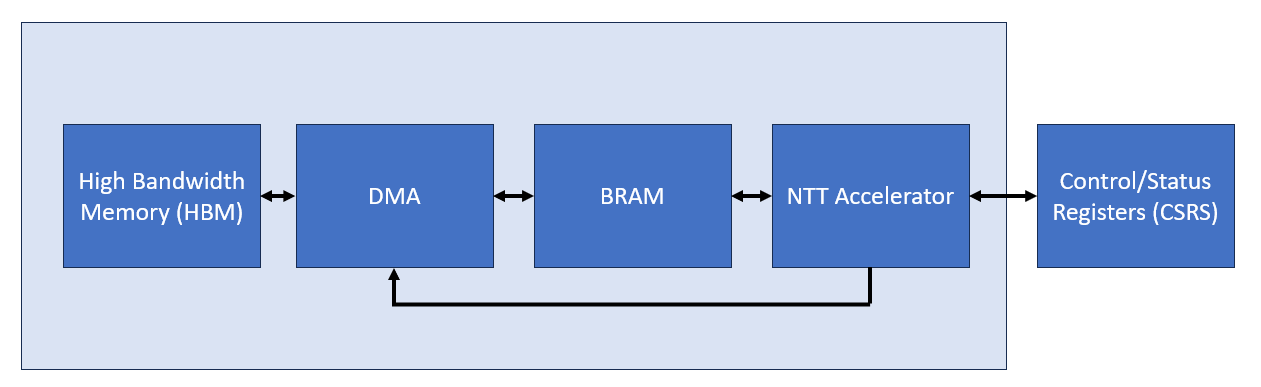
\includegraphics[width=0.9\textwidth]{img/memory_interface.png}
\caption{HBM interface for data transfer between DDR and BRAM}
\label{fig:mem_interface}
\end{figure}

\FloatBarrier

We did not get to implementing an interface for this thesis work. Instead, we verified the correctness in simulation where it takes only 85 clock cycles to move all data into the BRAMs. However, in simulation the speed is only limited by the bandwidth of the BRAMs, while in reality it is also limited by the HBM bandwidth. To achieve the same speed with a real memory interface it might be necessary to duplicate each BRAM and use it as buffer so memory can be transferred during the NTT computation. Nevertheless, memory bandwidth is probably not a bottleneck for performance.

\section{Results}

\subsection{Simulation Results}

For the Verilog simulation data was first read into the BRAMs from a file, then the full NTT was computed with the data present in BRAM. The simulation showed that a full NTT can be computed in 2957 clock cycles. This number is always the same regardless of the data or modulus used. 2392 clock cycles are spent in computing the FFTs using Cooley-Tukey's algorithm, 514 clock cycles in pointwise multiplication for Rader's algorithm and 51 cycles are pipeline stalls which corresponds to only 1.7\% of the execution time. Writing all data to the BRAMs and reading from them both takes 85 clock cycles. If we include this time the total latency for an NTT computation would be 2562 clock cycles.

\subsection{Implementation Results}

The implementation results are shown in Table \ref{table:implementation_results}. These results include the entire NTT but without external BRAM interface. 257 of the BRAMs are used as RAM, and 171 BRAMs are used as ROM to store the twiddle factors. The Alveo u250 FPGA contains BRAM tiles which can implement either one large BRAM or two smaller BRAMs. The 171 BRAMs used for ROM use one BRAM tile each, the 257 BRAMs used as RAM use only 128.5 BRAM tiles. Therefore utilization reports show only 299.5 BRAMs used.
\\\\
The implementation run with default settings in Vivado suffered from SLL (Super Long Line) congestion. SLLs connect signals between large regions called Super Logic Regions (SLR) on the FPGA. There are only a limited number of these connections available and the router has difficulty with timing closure when a high portion of these SLLs is used. To address this problem the placer directive SSI\_BalanceSLLs was used which eliminated the use of SLLs entirely by confining all the logic to one SLR. The single SLR placement solves the SLL congestion but introduced congestion on the connections within the SLR, therefore the clock frequency had to be lowered from 200 MHz in synthesis to 125 MHz after placement. The critical path in this design was simply a connection between two registers that contained no logic, this is a clear indication of routing problems.

\begin{table}[!h]
\caption{Implementation results}
\label{table:implementation_results}
\centering
\begin{tabular}{ *{5}{|c}| } 
 \hline
 Frequency (MHz) &  CLB LUT & CLB Register & BRAM  & DSP  \\ \hline
 125             &  230043  & 118765       & 299.5 & 1024 \\
 \hline
\end{tabular}
\end{table}

\FloatBarrier

\subsection{Comparison to other implementations}
Few efforts have been made in hardware acceleration of NTTs with non-power-of-two lengths. Wu, Chen and Shieh's implementation \cite{9937536} which employs Bluestein's algorithm to handle NTTs with non-power-of-two lengths. To the best of our knowledge, this is the only non-power-of-two implementation of comparable size. Their implementation can not be used for BGV-FHE in the same way since it supports only a single modulus. Despite this we will focus mostly on on Wu et al.'s implementation, since the other implementations are only suitable for power-of-two length NTTs. \cite{ozturk2574340, 10.1145/3373376.3378523, 9171507, cryptoeprint:2013/866, cryptoeprint:2020/446}

\begin{table}[h!]
\caption{Comparison to other implementation results.}
\label{table:implementation_comparison}
\centering
\resizebox{\textwidth}{!}{%
\begin{tabular}{ |m{0.18\textwidth}*{7}{|m{0.12\textwidth}}| } 
 \hline
 Design              & Proposed    & \cite{9937536} & \cite{ozturk2574340} & \cite{10.1145/3373376.3378523} & \cite{9171507} & \cite{cryptoeprint:2013/866} & \cite{cryptoeprint:2020/446} \\ \hline \hline
 NTT points          & 21845       & [4098..8193] & 32768    & 8192                & 4096     & 512      & 1024      \\  \hline
 Modulus size (bits) & 32          & 64           & 32       & 54                  & 60       & 13       & 16        \\  \hline
 Platform            & Alveo U250  & Virtex-7     & Virtex-7 & Stratix 10 GX 2800  & Virtex-7 & Virtex 6 & Arktix-7  \\  \hline
 Frequency (MHz)     & 125         & 250          & 250      & 300                 & 125      & 278      & 45.47     \\  \hline
 Cycles              & 2957        & 5825         & 12725    & 768                 & 972      & 2304     & 18537     \\  \hline
 CLB LUTs            & 230k        & 76.2k        & 219k     & 142k                & 99.3k    & 1536     & 2908      \\  \hline
 CLB Registers       & 118k        & /            & 90.7k    & 387k                & /        & 953      & 170       \\  \hline
 BRAM                & 299.5       & 62           & 193      & 725                 & 176      & 3        & 0         \\  \hline
 DSPs                & 1024        & 256          & 768      & 320                 & 929      & 1        & 9         \\                       
 \hline
\end{tabular}}
\end{table}

To facilitate performance comparison, Table \ref{table:implementation_comparison} presents the cycle count for one forward NTT computation normalized to $m=1024$ and $k=32$, where $k$ is the modulus size in bits. We assume quasilinear scaling with $m$ due to the FFT operation's time complexity. Linear performance scaling is assumed for $k$ as lowering the small moduli's bit-width in the BGV scheme roughly corresponds to a proportional increase in the number of vectors in DoubleCRT representation. The normalized cycle count $\tilde{c}$ is calculated as

\begin{equation}
\label{eq:norm_cycles}
\tilde{c}=\text{cycles}\cdot\frac{32 \cdot 1024 \log_2 1024}{k \cdot m \log_2 m}
\end{equation}

The table also includes the products of the normalized cycle count with the number of LUTs and DSPs, indicating better performance with lower values. It is important to not that it is not possible to achieve a completely fair comparison due to variations in parameter sets, target devices, and other limitations that these metrics do not account for.
\\\\
Wu et al.'s implementation performs better on this metric when a 8193-point NTT is considered, which would be the best case for their implementation. A practical parameter for BGV would be $n=4369$. \cite{9937536} In this case our design performs significantly better. It is important to note that Wu et al.'s design can not be used for DoubleCRT conversion since it uses a fixed modulus to greatly simplify modular reduction, the DSP count in our design would be halved if we could use the same method. Our design however, has the limitation that the reversed re-indexing step is not performed in hardware when the NTT is finished. This step can be performed in linear time and is not strictly required until we convert back from DoubleCRT representation, therefore it is not likely to cause significant overhead.
\\\\
It is worth noting that power-of-two size NTTs are expected to offer at least twice the performance, as computing an NTT of a non-power-of-two size using Rader's or Bluestein's algorithms requires performing both an NTT and an inverse NTT.

\begin{table}[h!]
\caption{Comparison to other implementation using normalized number of cycles ($\tilde{c}$).}
\label{table:performance_comparison}
\centering
\begin{tabular}{ |l|r|r|r|r| } 
 \hline
 Design & NTT-points & $\tilde{c}$ & $\tilde{c}$ $\times$ CLB LUTs &  $\tilde{c}$ $\times$ DSPs \\ \hline \hline 
 Proposed  & 21845 & 96.1	& 22\,116\,274 & 98\,465 \\ \hline 
 \cite{9937536} (best case) & 8193 & 280.0 & 21\,339\,663 & 71\,692 \\ \hline 
 \cite{9937536} (practical) & 4369 & 564.5 & 43\,013\,187 & 144\,506 \\ \hline 
 \cite{ozturk2574340} & $2^{15}$ & 265.1 & 58\,057\,813 & 203\,600 \\ \hline 
 \cite{10.1145/3373376.3378523} & $2^{13}$ & 73.8 & 6\,214\,017 & 14\,003 \\ \hline 
 \cite{9171507} & $2^{12}$ & 202.5 & 10\,724\,400 & 100\,332 \\ \hline 
 \cite{cryptoeprint:2013/866} & $2^{9}$ & 7651.1 & 19\,358\,326 & 12\,603 \\ \hline 
 \cite{cryptoeprint:2020/446} & $2^{10}$ & 18537 & 107\,811\,192 & 333\,666 \\ \hline
\end{tabular}
\end{table}

\FloatBarrier

\section{Conclusion}
This chapter focused on the hardware architecture and implementation of a 21845-point NTT. It addressed the challenges of efficiently implementing NTTs with non-power-of-two lengths, which are required for more efficient fully homomorphic encryption computation. The proposed hardware architecture utilized a combination of the Prime-Factor FFT algorithm and Rader's algorithm to efficiently compute the NTT.
\\\\
Simulation results showed that a complete 21845-point NTT computation could be performed in 2957 clock cycles. Implementation results on the Alveo U250 FPGA showed that the design utilized 230,043 LUTs and 118,765 registers. The design also used 299.5 BRAMs and required 1024 DSPs.
\\\\
Comparison with existing implementations highlighted the efficiency of the proposed design. In terms of normalized performance metrics, the proposed design performed competitively with respect to other implementations for various NTT sizes. Notably, the design demonstrated better performance for practical parameter sets, making it a promising choice for applications where the 21845-th cyclotomic can provide significant performance improvements, such as HElib's BGV Fully Homomorphic Encryption.


\chapter{Conclusion}

\section{Summary}
In this thesis, we presented a hardware architecture for efficient non-power-of-two number theoretic transform computations, targeting fully homomorphic encryption using the BGV scheme. We have shown that a combination of the Prime-Factor FFT algorithm and Rader's algorithm outperforms other algorithms when the bootstrappable parameters for HElib's BGV are considered. Our design focuses on the 21845-th cyclotomic polynomial, which is a practical parameter for BGV, and has ideal properties our design. We used efficient arithmetic and algorithmic optimization techniques and leveraged parallel processing, pipelining, optimized memory management and hardware reuse to achieve high throughput and efficient resource utilization. The simulation and implementation results have demonstrated competitive performance as compared to existing implementations for both power-of-two and non-power-of-two NTT sizes.

\section{Future Work}
In order to transform the prototype outlined within this thesis into a functional hardware implementation, the foremost task is to implement an interface that enables read and write operations to the memory on the FPGA.
\\\\
Further improvements are possible to optimize the design. While the existing configuration uses radix-2 butterflies, it is noteworthy that all NTTs computed via Cooley-Tukey's algorithm are of a power-of-four size, thereby warranting the use of radix-4 butterflies. Using radix-4 butterflies would lead to halving the number of NTT stages, with only a 50\% increment in the number of DSPs. Moreover, this modification would lead to a more efficient use of the permutation logic and memory, as their fixed area cost remains the same while the throughput increases. Alternatively, two stages of radix-2 butterflies can be used in series, doubling the number of butterfly units. While this might not improve the throughput relative to the number of DSPs, it would still halve the overhead of the permutation logic and memory. 
\\\\
The choice was made to use the Montgomery modular multiplier presented by Mert et al. \cite{9171507} and precompute all twiddle factors because it is convenient. However, it is important to acknowledge that this may not be the most optimal implementation. Another, less straightforward optimization was proposed by Hsu and Shieh \cite{9181192} which reduces the number of NTTs that need to be computed for PFA by eliminating redundant outputs. Finally, the design suffered from routing congestion. This might be alleviated with more optimal placement strategies.
\\\\
Software libraries, notably HElib, can benefit from the NTT accelerator for the transformation of polynomials into DoubleCRT form. Given that the hardware only offers native support for forward NTT computation, the elements in the DoubleCRT vector would need to be rearranged first in software. Integrating an hardware accelerator with a software library would be an interesting direction for future work.

\appendixpage*
\appendix
\chapter{Paper}
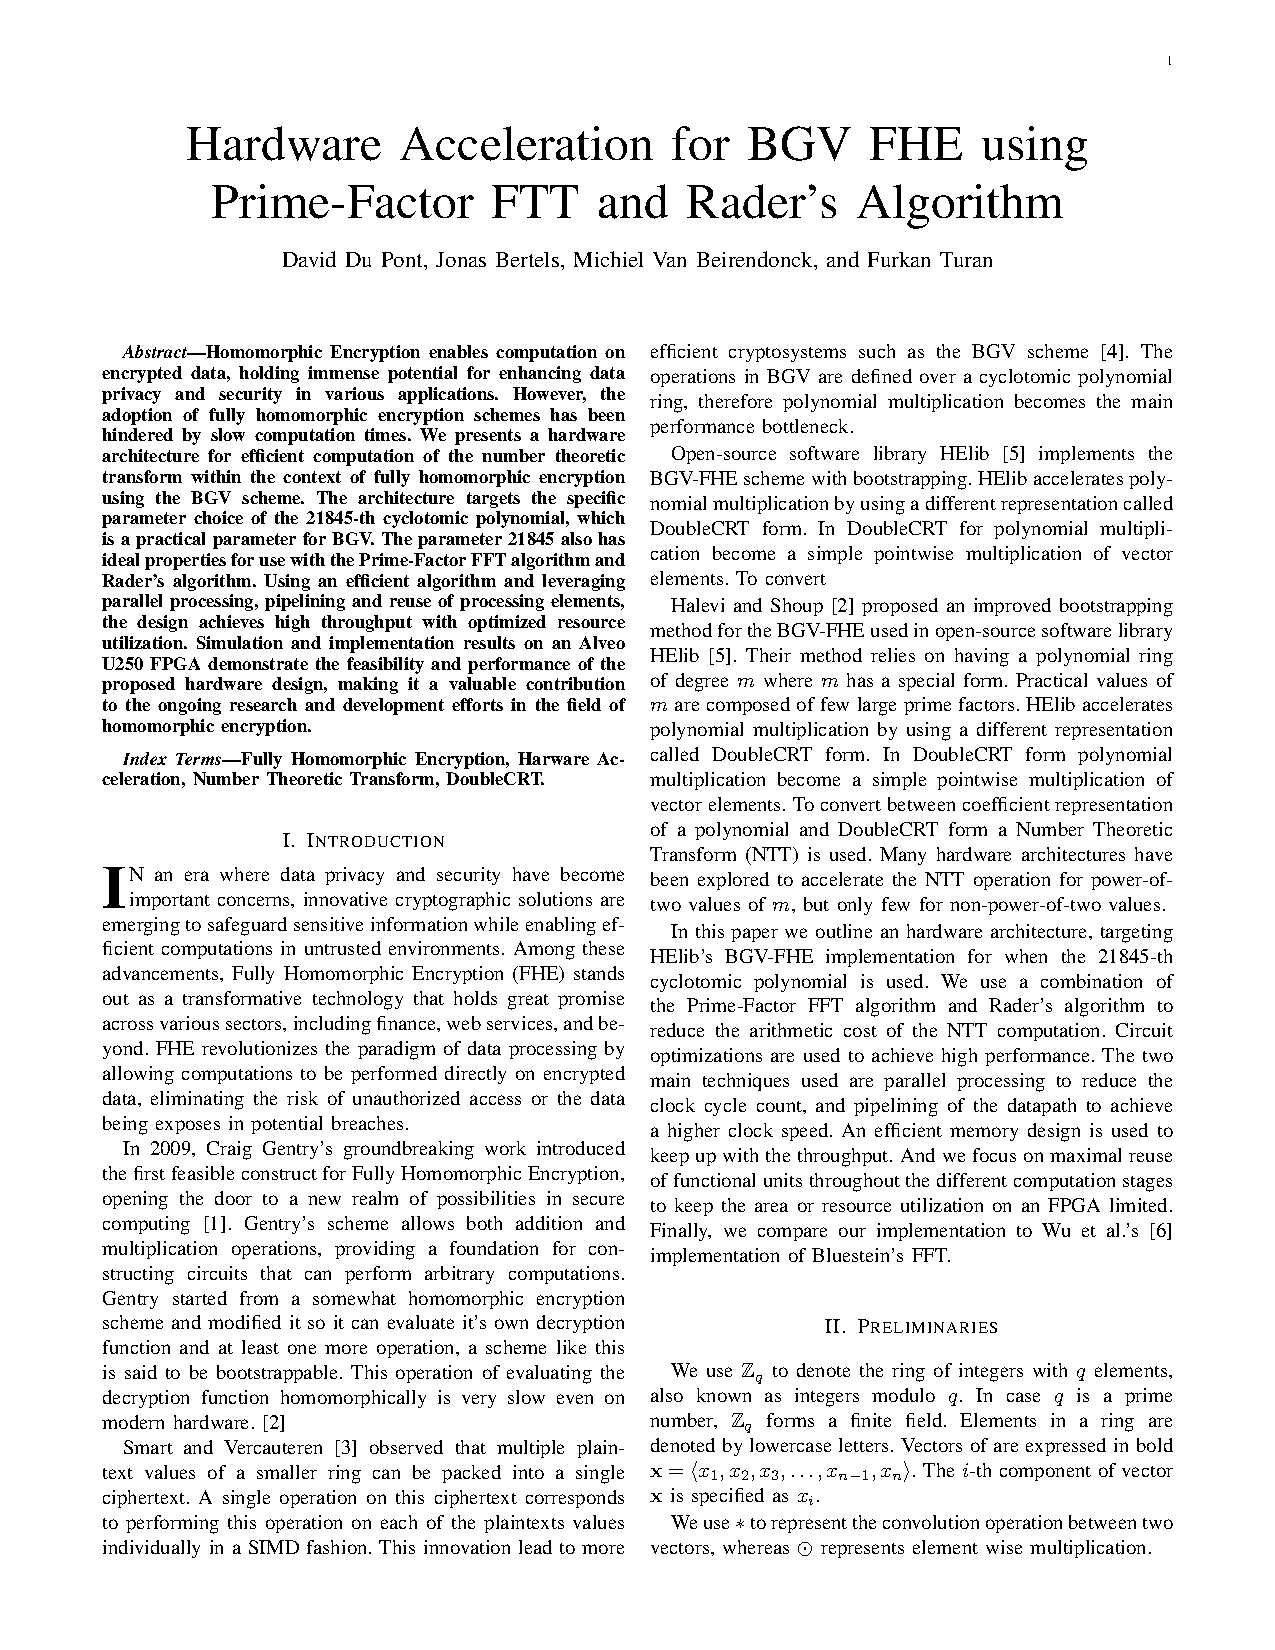
\includepdf[pages=-]{paper.pdf}  

\backmatter

\bibliographystyle{abbrv}
\bibliography{references}

\end{document}

